%%%%%%%%%%%%%%%%%%%%%%%%%%%%%%%%%%%%%%%%%%%%%%%%%%%%%%
% ARTÍCULO CIENTÍFICO - ANÁLISIS DE REGRESIÓN
% ---------------------------------------------------
% COMPILAR CON XeLaTeX (las fuentes usan fontspec).
% En Overleaf: Menú > Compilador > XeLaTeX.
%%%%%%%%%%%%%%%%%%%%%%%%%%%%%%%%%%%%%%%%%%%%%%%%%%%%%%

\documentclass[12pt,letterpaper]{article}

%%%%%%%%%%%%%%%%%%%%%%%%%%%%%%%%%%%%%%%%%%%%%%%%%%%%%%
% DATOS DEL TRABAJO
% ---------------------------------------------------
% Todo lo que cambia de un trabajo a otro está aquí:
% la portada, el título del artículo y el encabezado
% leen estos comandos. No hay que tocar nada más.
%%%%%%%%%%%%%%%%%%%%%%%%%%%%%%%%%%%%%%%%%%%%%%%%%%%%%%

% --- Título (español) y título en inglés -------------
\newcommand{\titulo}{Modelos de regresión para la eficiencia hidráulica de rodetes Pelton y Turgo de eje vertical}
\newcommand{\tituloingles}{Regression models for the hydraulic efficiency of vertical-axis Pelton and Turgo runners}

% Título corto para el encabezado de las páginas
\newcommand{\titulocorto}{Eficiencia hidráulica de rodetes Pelton y Turgo}

% --- Tipo de trabajo (sale en la portada) -------------
\newcommand{\tipotrabajo}{ARTÍCULO CIENTÍFICO}

% --- Curso --------------------------------------------
\newcommand{\materia}{Análisis de Regresión}
\newcommand{\semestre}{2026-2}
\newcommand{\codigo}{0000000}   % <- PENDIENTE: código de la asignatura
\newcommand{\departamento}{DEPARTAMENTO\\ DE ESTADÍSTICA}

% --- Autores ------------------------------------------
% Portada: un nombre por línea
\newcommand{\autoresportada}{%
María Paula Ardila Otero
% \\[0.2cm] Nombre del segundo integrante
}

% Primera página del artículo: nombre con superíndice
\newcommand{\autoresarticulo}{%
María Paula Ardila Otero$^{1,*}$
% , Nombre Apellido$^{1}$
}

% Afiliaciones (una por línea, mismo número del superíndice)
\newcommand{\afiliaciones}{%
$^{1}$Estudiante de Ciencias de la Computación y Estadística, Universidad Nacional de Colombia sede Medellín, Medellín, Colombia.\\
$^{*}$Autora de correspondencia:
\href{mailto:mardilao@unal.edu.co}{\texttt{mardilao@unal.edu.co}}%
}

% --- Profesor -----------------------------------------
\newcommand{\profesor}{Freddy Hernández Barajas}

% --- Repositorio con datos y código -------------------
\newcommand{\repositorio}{https://github.com/mariasaurius/Articulo_regresion}
         
%%%%%%%%%%%%%%%%%%%%%%%%%%%%%%%%%%%%%%%%%%%%%%%%%%%%%%
% IDIOMA
%%%%%%%%%%%%%%%%%%%%%%%%%%%%%%%%%%%%%%%%%%%%%%%%%%%%%%

% es-tabla       -> "Tabla" en vez de "Cuadro"
% es-nodecimaldot -> el punto decimal se queda como punto (igual que en R)
% es-noquoting   -> evita conflictos de < y > con TikZ
\usepackage[english,spanish,es-tabla,es-nodecimaldot,es-noquoting]{babel}

%%%%%%%%%%%%%%%%%%%%%%%%%%%%%%%%%%%%%%%%%%%%%%%%%%%%%%
% GEOMETRÍA
%%%%%%%%%%%%%%%%%%%%%%%%%%%%%%%%%%%%%%%%%%%%%%%%%%%%%%

\usepackage[
top=0.65in,
bottom=0.65in,
left=0.65in,
right=0.65in
]{geometry}

%%%%%%%%%%%%%%%%%%%%%%%%%%%%%%%%%%%%%%%%%%%%%%%%%%%%%%
% ENCABEZADO Y PIE DE PÁGINA (estilo artículo)
%%%%%%%%%%%%%%%%%%%%%%%%%%%%%%%%%%%%%%%%%%%%%%%%%%%%%%

\usepackage{fancyhdr}
\setlength{\headheight}{15pt}

% Páginas normales: título corto a la izquierda,
% curso a la derecha y línea roja, como en la revista
\pagestyle{fancy}
\fancyhf{}
\fancyhead[L]{\footnotesize\AncizarSansRegular\color{grisOscuroUN}\titulocorto}
\fancyhead[R]{\footnotesize\AncizarSansRegular\color{grisOscuroUN}\materia\ \textbullet\ \semestre}
\fancyfoot[C]{\AncizarSansRegular\thepage}
\renewcommand{\headrulewidth}{0.6pt}
\renewcommand{\headrule}{{\color{rojoUN}\hrule width\headwidth height\headrulewidth}}

% Primera página del artículo: solo el número de página
\fancypagestyle{plain}{%
  \fancyhf{}
  \fancyfoot[C]{\AncizarSansRegular\thepage}
  \renewcommand{\headrulewidth}{0pt}%
}


%%%%%%%%%%%%%%%%%%%%%%%%%%%%%%%%%%%%%%%%%%%%%%%%%%%%%%
% FUENTES
%%%%%%%%%%%%%%%%%%%%%%%%%%%%%%%%%%%%%%%%%%%%%%%%%%%%%%

\usepackage{fontspec}
\usepackage{microtype}

%%%%%%%%%%%%%%%%%%%%%%%%%%%%%%%%%%%%%%%%%%%%%%%%%%%%%%
% MATEMÁTICAS
%%%%%%%%%%%%%%%%%%%%%%%%%%%%%%%%%%%%%%%%%%%%%%%%%%%%%%

\usepackage{amsmath}
\usepackage{amssymb}
\usepackage{amsthm}
\usepackage{cancel}
\usepackage{bm}        % letras griegas en negrita: \bm{\beta}

%%%%%%%%%%%%%%%%%%%%%%%%%%%%%%%%%%%%%%%%%%%%%%%%%%%%%%
% GRÁFICOS Y TABLAS
%%%%%%%%%%%%%%%%%%%%%%%%%%%%%%%%%%%%%%%%%%%%%%%%%%%%%%

\usepackage{graphicx}
\usepackage{booktabs}
\usepackage{tabularx}
\usepackage{multirow}
\usepackage{multicol}
\usepackage{float}
\usepackage{pdflscape}

%%%%%%%%%%%%%%%%%%%%%%%%%%%%%%%%%%%%%%%%%%%%%%%%%%%%%%
% COLORES
%%%%%%%%%%%%%%%%%%%%%%%%%%%%%%%%%%%%%%%%%%%%%%%%%%%%%%

\usepackage[dvipsnames,table]{xcolor}
\usepackage{colortbl}
%==================================================
% COLORES INSTITUCIONALES UNAL
%==================================================

\definecolor{verdeUN}{RGB}{148,180,59}      % Pantone 376C
\definecolor{rojoUN}{RGB}{166,28,49}        % Pantone 187C
\definecolor{rojoOscuroUN}{RGB}{118,35,47}  % Pantone 188C
\definecolor{verdeOscuroUN}{RGB}{70,107,63} % Pantone 7743C
\definecolor{grisOscuroUN}{RGB}{86,90,92}   % Pantone 425C
\definecolor{grisClaroUN}{RGB}{177,178,176} % Pantone 421C

%==================================================
% COLORES PARA CÓDIGO
%==================================================

\definecolor{bgcream}{HTML}{FFF8E7}
\definecolor{keywordcolor}{RGB}{70,107,63}
\definecolor{stringcolor}{RGB}{166,28,49}
\definecolor{commentcolor}{RGB}{86,90,92}

%%%%%%%%%%%%%%%%%%%%%%%%%%%%%%%%%%%%%%%%%%%%%%%%%%%%%%
% TIKZ
%%%%%%%%%%%%%%%%%%%%%%%%%%%%%%%%%%%%%%%%%%%%%%%%%%%%%%

\usepackage{tikz}

%%%%%%%%%%%%%%%%%%%%%%%%%%%%%%%%%%%%%%%%%%%%%%%%%%%%%%
% HIPERVÍNCULOS
%%%%%%%%%%%%%%%%%%%%%%%%%%%%%%%%%%%%%%%%%%%%%%%%%%%%%%

\usepackage{xurl}
\usepackage[hidelinks]{hyperref}

%%%%%%%%%%%%%%%%%%%%%%%%%%%%%%%%%%%%%%%%%%%%%%%%%%%%%%
% REFERENCIAS (igual que la plantilla del profesor)
%%%%%%%%%%%%%%%%%%%%%%%%%%%%%%%%%%%%%%%%%%%%%%%%%%%%%%
% \citet{clave}  -> Autor (año)
% \citep{clave}  -> (Autor, año)

%\usepackage[round]{natbib}
%\bibliographystyle{abbrvnat-es}   % abbrvnat en español (archivo abbrvnat-es.bst)
%\setlength{\bibsep}{4pt}

%%%%%%%%%%%%%%%%%%%%%%%%%%%%%%%%%%%%%%%%%%%%%%%%%%%%%%
% CAJAS
%%%%%%%%%%%%%%%%%%%%%%%%%%%%%%%%%%%%%%%%%%%%%%%%%%%%%%

\usepackage[most]{tcolorbox}

%%%%%%%%%%%%%%%%%%%%%%%%%%%%%%%%%%%%%%%%%%%%%%%%%%%%%%
% CAPTIONS Y LISTAS
%%%%%%%%%%%%%%%%%%%%%%%%%%%%%%%%%%%%%%%%%%%%%%%%%%%%%%

\usepackage{caption}
\usepackage{enumitem}

\captionsetup{font=small, labelfont=bf, labelsep=period, margin=0.5cm}
\setlength{\belowcaptionskip}{6pt}

%%%%%%%%%%%%%%%%%%%%%%%%%%%%%%%%%%%%%%%%%%%%%%%%%%%%%%
% NÚMEROS
%%%%%%%%%%%%%%%%%%%%%%%%%%%%%%%%%%%%%%%%%%%%%%%%%%%%%%

\usepackage{siunitx}

\sisetup{
table-number-alignment = center,
input-symbols = {+},
table-space-text-post = {+}
}

%%%%%%%%%%%%%%%%%%%%%%%%%%%%%%%%%%%%%%%%%%%%%%%%%%%%%%
% SECCIONES
%%%%%%%%%%%%%%%%%%%%%%%%%%%%%%%%%%%%%%%%%%%%%%%%%%%%%%

\usepackage{titlesec}

\titleformat{\section}
{\Large\bfseries}
{\thesection.}{0.5em}{}
[\vspace{0.3em}\color{rojoUN}\titlerule]

\titleformat{\subsection}
{\large\bfseries\color{verdeOscuroUN}}
{\thesubsection.}{0.5em}{}

\titleformat{\subsubsection}
{\normalsize\bfseries\itshape}
{\thesubsubsection.}{0.5em}{}

\titlespacing*{\section}{0pt}{2.2ex plus 0.5ex}{1.2ex}
\titlespacing*{\subsection}{0pt}{1.8ex plus 0.5ex}{0.8ex}

%%%%%%%%%%%%%%%%%%%%%%%%%%%%%%%%%%%%%%%%%%%%%%%%%%%%%%
% COLORBOX
%%%%%%%%%%%%%%%%%%%%%%%%%%%%%%%%%%%%%%%%%%%%%%%%%%%%%%

\newtcolorbox{cuadro_verde}[1]{
    enhanced,
    breakable,
    colback=white,
    colframe=verdeUN,
    colbacktitle=verdeUN,
    coltitle=white,
    fonttitle=\AncizarSansSemiBold,
    title=#1,
    boxrule=0.8pt,
    arc=2mm,
    left=3mm,
    right=3mm,
    top=2mm,
    bottom=2mm
}

\newtcolorbox{cuadro_verdeOscuro}[1]{
    enhanced,
    breakable,
    colback=white,
    colframe=verdeOscuroUN,
    colbacktitle=verdeOscuroUN,
    coltitle=white,
    fonttitle=\AncizarSansSemiBold,
    title=#1,
    boxrule=0.8pt,
    arc=2mm,
    left=3mm,
    right=3mm,
    top=2mm,
    bottom=2mm
}

\newtcolorbox{cuadro_rojo}[1]{
    enhanced,
    breakable,
    colback=white,
    colframe=rojoUN,
    colbacktitle=rojoUN,
    coltitle=white,
    fonttitle=\AncizarSansSemiBold,
    title=#1,
    boxrule=0.8pt,
    arc=2mm,
    left=3mm,
    right=3mm,
    top=2mm,
    bottom=2mm
}

\newtcolorbox{cuadro_rojo_Oscuro}[1]{
    enhanced,
    breakable,
    colback=white,
    colframe=rojoOscuroUN,
    colbacktitle=rojoOscuroUN,
    coltitle=white,
    fonttitle=\AncizarSansSemiBold,
    title=#1,
    boxrule=0.8pt,
    arc=2mm,
    left=3mm,
    right=3mm,
    top=2mm,
    bottom=2mm
}

\newtcolorbox{cuadro_grisClaro}[1]{
    enhanced,
    breakable,
    colback=white,
    colframe=grisClaroUN,
    colbacktitle=grisClaroUN,
    coltitle=white,
    fonttitle=\AncizarSansSemiBold,
    title=#1,
    boxrule=0.8pt,
    arc=2mm,
    left=3mm,
    right=3mm,
    top=2mm,
    bottom=2mm
}

\newtcolorbox{cuadro_grisOscuro}[1]{
    enhanced,
    breakable,
    colback=white,
    colframe=grisOscuroUN,
    colbacktitle=grisOscuroUN,
    coltitle=white,
    fonttitle=\AncizarSansSemiBold,
    title=#1,
    boxrule=0.8pt,
    arc=2mm,
    left=3mm,
    right=3mm,
    top=2mm,
    bottom=2mm
}


\newtcolorbox{nota}{
    enhanced,
    breakable,
    colback=white,
    colframe=verdeUN,
    borderline west={3pt}{0pt}{verdeUN},
    boxrule=0pt,
    arc=0mm,
    left=5mm,
    right=3mm,
    top=2mm,
    bottom=2mm
}


%%%%%%%%%%%%%%%%%%%%%%%%%%%%%%%%%%%%%%%%%%%%%%%%%%%%%%
% LISTINGS
%%%%%%%%%%%%%%%%%%%%%%%%%%%%%%%%%%%%%%%%%%%%%%%%%%%%%%

%%%%%%%%%%%%%%%%%%%%%%%%%%%%%%%%%%%%%%%%%%%%%%%%%%%%%%
% FUENTE JETBRAINS MONO
%%%%%%%%%%%%%%%%%%%%%%%%%%%%%%%%%%%%%%%%%%%%%%%%%%%%%%

% Usa IBM Plex Mono si está instalada; si no (por ejemplo
% en otro computador), usa la JetBrains Mono que viene en
% Config/Fuentes, para que el documento siempre compile.
\IfFontExistsTF{IBM Plex Mono}{%
  \setmonofont{IBM Plex Mono}%
}{%
  \setmonofont{JetBrainsMono}[
  Path=Config/Fuentes/JetBrains/,
  Extension=.ttf,
  UprightFont=*-Regular,
  ItalicFont=*-Italic,
  BoldFont=JetBrainsMonoNL-Bold,
  BoldItalicFont=JetBrainsMonoNL-BoldItalic,
  Scale=0.9
  ]%
}


\usepackage{listings}

\lstdefinestyle{Rcode}{
language=R,
backgroundcolor=\color{bgcream},
keywordstyle=\color{keywordcolor}\bfseries,
commentstyle=\color{commentcolor}\itshape,
stringstyle=\color{stringcolor},
basicstyle=\fontsize{10}{14}\ttfamily\selectfont,
numbers=left,
numberstyle=\footnotesize\color{grisClaroUN},
numbersep=8pt,
frame=single,
rulecolor=\color{grisClaroUN},
breaklines=true,
showstringspaces=false,
morekeywords={library,ggplot,df2,zcounts},
xleftmargin=10pt,
framesep=6pt
}

\lstdefinestyle{Routput}{
basicstyle=\fontsize{10}{14}\ttfamily\selectfont,
backgroundcolor=\color{white},
frame=single,
rulecolor=\color{grisClaroUN},
breaklines=true,
showstringspaces=false,
numbers=none,
xleftmargin=10pt,
framesep=6pt
}

%%%%%%%%%%%%%%%%%%%%%%%%%%%%%%%%%%%%%%%%%%%%%%%%%%%%%%
% FUENTE PRINCIPAL DEL DOCUMENTO (SERIF)
%%%%%%%%%%%%%%%%%%%%%%%%%%%%%%%%%%%%%%%%%%%%%%%%%%%%%%

% (sintaxis estándar de fontspec: funciona también con
% versiones de TeX Live más viejas)
\setmainfont{AncizarSerif}[
Path=Config/Fuentes/Serif/,
Extension=.ttf,
UprightFont=*-Regular,
ItalicFont=*-Italic,
BoldFont=*-Bold,
BoldItalicFont=*-BoldItalic
]

%%%%%%%%%%%%%%%%%%%%%%%%%%%%%%%%%%%%%%%%%%%%%%%%%%%%%%
% FUENTES SANS (PORTADA)
%%%%%%%%%%%%%%%%%%%%%%%%%%%%%%%%%%%%%%%%%%%%%%%%%%%%%%

\newfontfamily\AncizarSansMedium[
Path=Config/Fuentes/Sans/
]
{AncizarSans-Medium.ttf}

\newfontfamily\AncizarSansLight[
Path=Config/Fuentes/Sans/
]
{AncizarSans-Light.ttf}

\newfontfamily\AncizarSansLightItalic[
Path=Config/Fuentes/Sans/
]
{AncizarSans-LightItalic.ttf}

\newfontfamily\AncizarSansRegular[
Path=Config/Fuentes/Sans/
]
{AncizarSans-Regular.ttf}

\newfontfamily\AncizarSansSemiBold[
Path=Config/Fuentes/Sans/
]
{AncizarSans-SemiBold.ttf}

\newfontfamily\AncizarSansExtraBold[
Path=Config/Fuentes/Sans/
]
{AncizarSans-ExtraBold.ttf}

%%%%%%%%%%%%%%%%%%%%%%%%%%%%%%%%%%%%%%%%%%%%%%%%%%%%%%
% FUENTES SERIF AUXILIARES
%%%%%%%%%%%%%%%%%%%%%%%%%%%%%%%%%%%%%%%%%%%%%%%%%%%%%%

\newfontfamily\AncizarSerifMedium[
Path=Config/Fuentes/Serif/
]
{AncizarSerif-Medium.ttf}

\newfontfamily\AncizarSerifLight[
Path=Config/Fuentes/Serif/
]
{AncizarSerif-Light.ttf}

\newfontfamily\AncizarSerifLightItalic[
Path=Config/Fuentes/Serif/
]
{AncizarSerif-LightItalic.ttf}

\newfontfamily\AncizarSerifRegular[
Path=Config/Fuentes/Serif/
]
{AncizarSerif-Regular.ttf}

\newfontfamily\AncizarSerifSemiBold[
Path=Config/Fuentes/Serif/
]
{AncizarSerif-SemiBold.ttf}

\newfontfamily\AncizarSerifExtraBold[
Path=Config/Fuentes/Serif/
]
{AncizarSerif-ExtraBold.ttf}

%%%%%%%%%%%%%%%%%%%%%%%%%%%%%%%%%%%%%%%%%%%%%%%%%%%%%%
% RESUMEN Y ABSTRACT (estructura de la plantilla
% del profesor, con el estilo de cajas de la mía)
%%%%%%%%%%%%%%%%%%%%%%%%%%%%%%%%%%%%%%%%%%%%%%%%%%%%%%
% Uso:
% \begin{resumen}
%   texto...
%   \palabrasclave{palabra 1, palabra 2}
% \end{resumen}

\newcommand{\palabrasclave}[1]{%
  \par\medskip\noindent{\AncizarSansSemiBold\color{rojoUN}Palabras clave:}\ #1.}
\newcommand{\keywords}[1]{%
  \par\medskip\noindent{\AncizarSansSemiBold\color{rojoUN}Keywords:}\ #1.}

\newtcolorbox{cajaresumen}[1]{
    enhanced,
    breakable,
    colback=white,
    colframe=verdeUN,
    borderline west={3pt}{0pt}{verdeUN},
    boxrule=0pt,
    arc=0mm,
    left=5mm, right=3mm, top=2mm, bottom=2mm,
    fontupper=\small,
    title={#1},
    coltitle=rojoUN,
    colbacktitle=white,
    fonttitle=\AncizarSansSemiBold\large,
    attach title to upper={\par\smallskip}
}

\newenvironment{resumen}{\begin{cajaresumen}{Resumen}}{\end{cajaresumen}}
\renewenvironment{abstract}{\begin{cajaresumen}{Abstract}\selectlanguage{english}}{\end{cajaresumen}}

%%%%%%%%%%%%%%%%%%%%%%%%%%%%%%%%%%%%%%%%%%%%%%%%%%%%%%
% MODO BORRADOR: notas de lo que falta
%%%%%%%%%%%%%%%%%%%%%%%%%%%%%%%%%%%%%%%%%%%%%%%%%%%%%%
% \pendiente{...} muestra una caja roja mientras
% \borradortrue esté activo en main.tex. Con
% \borradorfalse desaparecen todas de una vez.

\newif\ifborrador
\borradortrue

\newcommand{\pendiente}[1]{%
  \ifborrador
  \begin{cuadro_rojo}{Pendiente}#1\end{cuadro_rojo}%
  \fi}

% Enlace al repositorio (el texto viene de Config/datos.tex)
\newcommand{\enlacerepositorio}{\expandafter\url\expandafter{\repositorio}}

% Parámetros de las figuras flotantes: permiten poner figuras grandes
% junto con texto en la misma página (menos páginas medio vacías)
\renewcommand{\topfraction}{0.9}
\renewcommand{\bottomfraction}{0.8}
\renewcommand{\textfraction}{0.07}
\renewcommand{\floatpagefraction}{0.75}
\setcounter{topnumber}{3}
\setcounter{totalnumber}{4}

% Las figuras no se salen de su sección (no terminan después de las referencias)
\usepackage[section]{placeins}

%%%%%%%%%%%%%%%%%%%%%%%%%%%%%%%%%%%%%%%%%%%%%%%%%%%%%%
% PRIMERA PÁGINA DEL ARTÍCULO
% ---------------------------------------------------
% Mismos elementos que la plantilla del profesor
% (título, título en inglés, autores, afiliaciones),
% con el encabezado UNAL de mi portada.
% Los textos salen de Config/datos.tex
%%%%%%%%%%%%%%%%%%%%%%%%%%%%%%%%%%%%%%%%%%%%%%%%%%%%%%

\newcommand{\tituloarticulo}{%
\thispagestyle{plain}%
\noindent
\begin{tikzpicture}
  % Logo
  \node[anchor=west, inner sep=0pt] (logo) at (0,0)
    {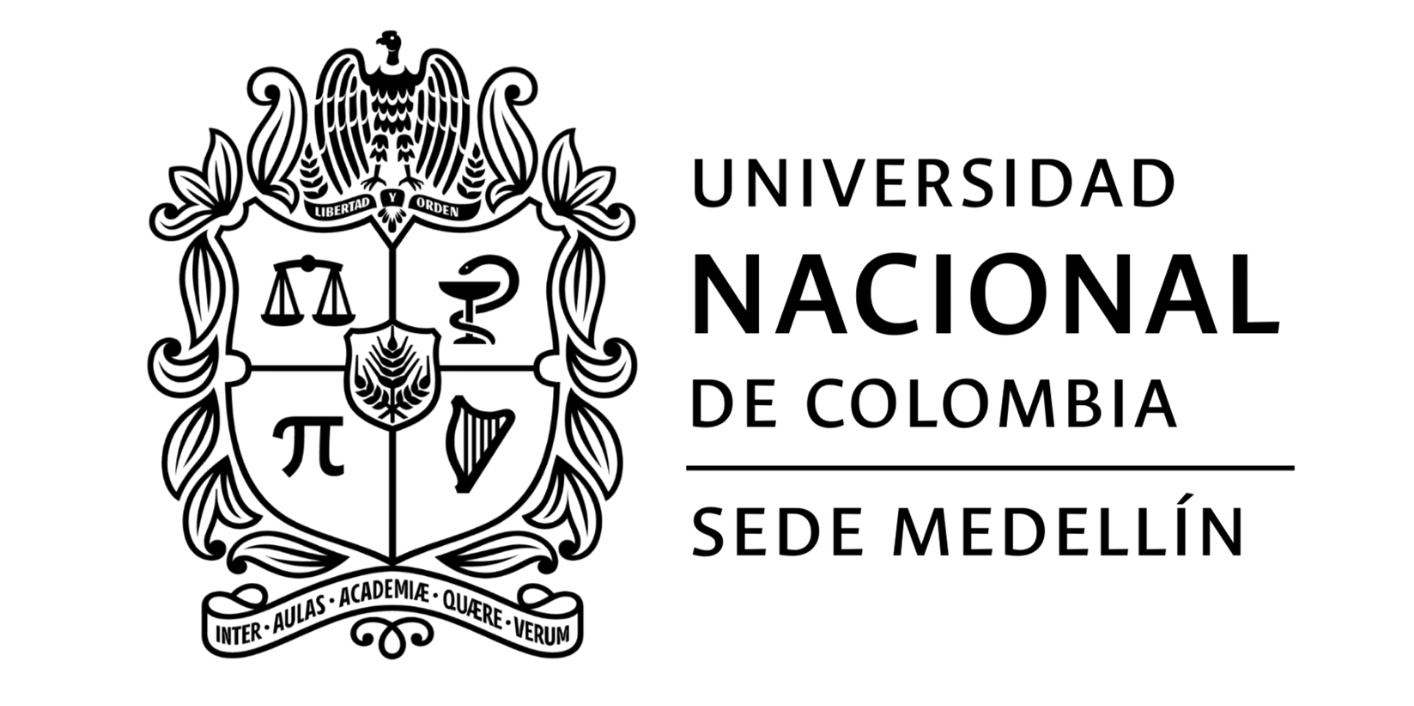
\includegraphics[height=1.5cm]{Imágenes/logo_unal.png}};
  % Línea vertical
  \draw[color=grisClaroUN, line width=0.6pt]
    ([xshift=0.45cm,yshift=-0.15cm]logo.north east) --
    ([xshift=0.45cm,yshift=0.15cm]logo.south east);
  % Departamento
  \node[anchor=west, align=left, font=\AncizarSansMedium\footnotesize,
        xshift=0.85cm] at (logo.east) {\departamento};
  % Curso y semestre a la derecha
  \node[anchor=east, align=right, font=\AncizarSansLightItalic\footnotesize,
        text=grisOscuroUN] at (\textwidth,0)
    {\materia\\ Semestre \semestre};
\end{tikzpicture}
\par\vspace{1.1cm}
%
% Título
{\raggedright\AncizarSansSemiBold\fontsize{24}{29}\selectfont
 \color{rojoUN}\titulo\par}
\vspace{0.35cm}
{\color{verdeUN}\rule{4cm}{1.8pt}}\par
\vspace{0.3cm}
% Título en inglés (el "subtitle" de la plantilla del profesor)
{\raggedright\AncizarSansLightItalic\fontsize{14}{18}\selectfont
 \color{grisOscuroUN}\tituloingles\par}
\vspace{0.7cm}
%
% Autores y afiliaciones
{\AncizarSansMedium\large\autoresarticulo\par}
\vspace{0.2cm}
{\footnotesize\color{grisOscuroUN}\afiliaciones\par}
\vspace{0.25cm}
{\footnotesize{\AncizarSansLightItalic\color{rojoUN}Profesor:}\ \profesor\par}
\vspace{0.6cm}
}


% ---------------------------------------------------
% INTERRUPTORES
% ---------------------------------------------------
\newif\ifportada
\portadafalse     % \portadatrue para poner mi portada al inicio
\newif\ifindice
\indicefalse      % \indicetrue para poner tabla de contenido
\borradorfalse    % \borradortrue muestra las cajas "Pendiente"

\begin{document}

% ---------------- Portada opcional ----------------
\ifportada
  % Portada: los textos salen de Config/datos.tex
\thispagestyle{empty}

\begin{tikzpicture}[remember picture,overlay]

%%%%%%%%%%%%%%%%%%%%%%%%%%%%%%%%%%%%%%%%%%%%%%%%%%%%%%
% MARCA DE AGUA
%%%%%%%%%%%%%%%%%%%%%%%%%%%%%%%%%%%%%%%%%%%%%%%%%%%%%%

\node[
anchor=south east,
opacity=0.05,
inner sep=0pt
]
at ([xshift=-0.5cm,yshift=0.5cm]current page.south east)
{
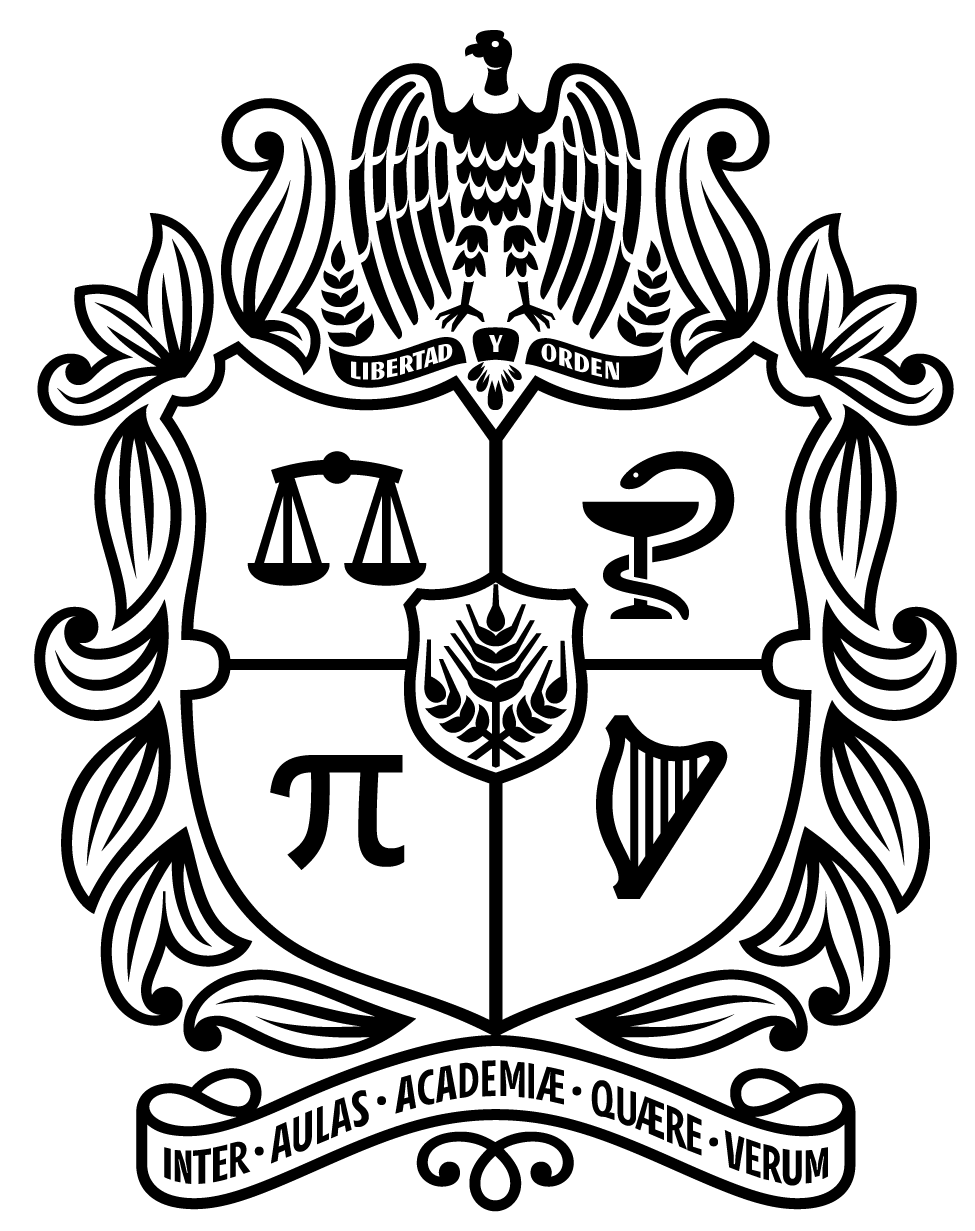
\includegraphics[width=10cm]
{Imágenes/escudo_marca_agua.png}
};

%%%%%%%%%%%%%%%%%%%%%%%%%%%%%%%%%%%%%%%%%%%%%%%%%%%%%%
% ENCABEZADO
%%%%%%%%%%%%%%%%%%%%%%%%%%%%%%%%%%%%%%%%%%%%%%%%%%%%%%

\node[
anchor=north west,
xshift=1.8cm,
yshift=-1.8cm
]
(logo)
at (current page.north west)
{
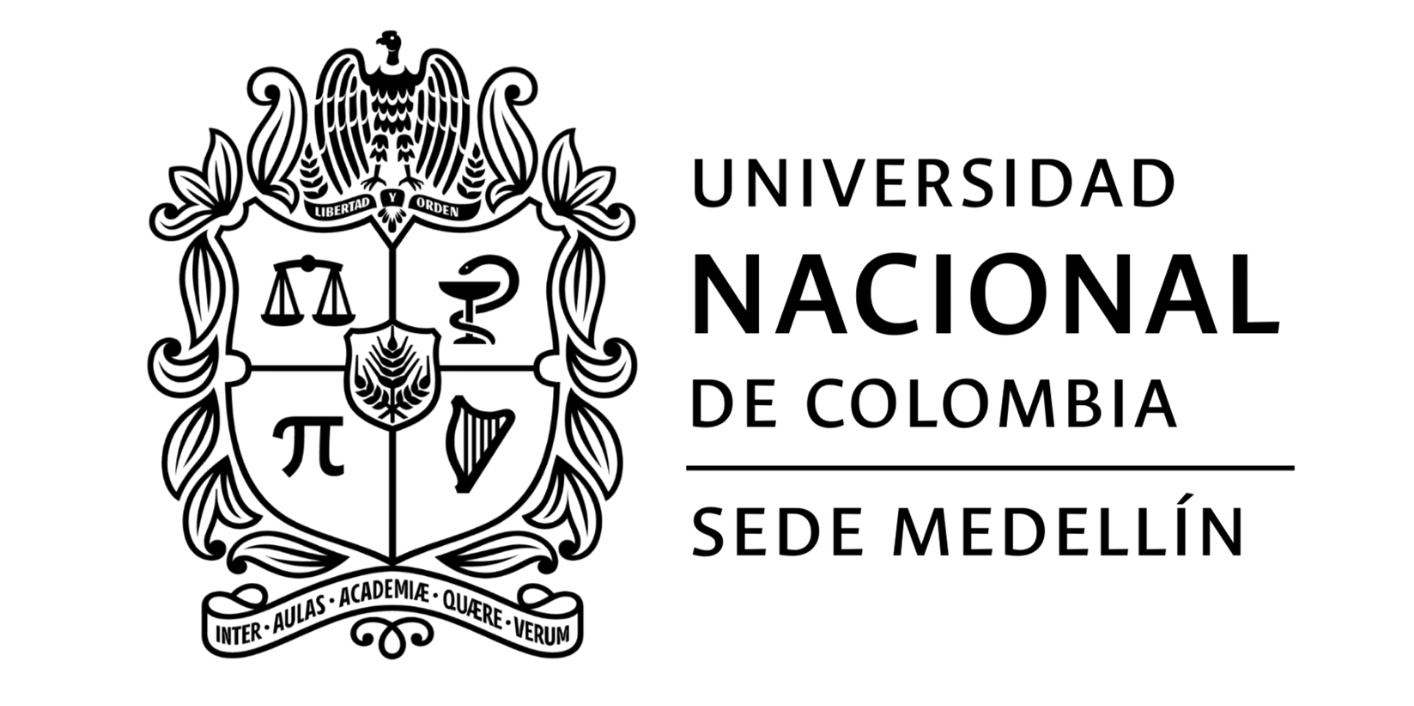
\includegraphics[height=2.8cm]
{Imágenes/logo_unal.png}
};

% Línea vertical
\draw[
color=grisClaroUN,
line width=0.6pt
]
([xshift=0.55cm,yshift=-0.25cm]logo.north east)
--
([xshift=0.55cm,yshift=0.25cm]logo.south east);

% Departamento
\node[ anchor=west, align=left, font=\AncizarSansMedium\small, text=black, xshift=1cm ] at (logo.east) { \departamento };

%%%%%%%%%%%%%%%%%%%%%%%%%%%%%%%%%%%%%%%%%%%%%%%%%%%%%%
% CONTENIDO
%%%%%%%%%%%%%%%%%%%%%%%%%%%%%%%%%%%%%%%%%%%%%%%%%%%%%%

\coordinate (inicioTexto)
at ([xshift=2.2cm,yshift=-10cm]
current page.north west);

\node[
anchor=west,
font=\AncizarSansSemiBold\fontsize{46}{50}\selectfont,
text=rojoUN
]
(titulo)
at (inicioTexto)
{
\tipotrabajo
};

\draw[
color=verdeUN,
line width=1.8pt
]
([yshift=-0.45cm]titulo.south west)
--
([xshift=15cm,yshift=-0.45cm]
titulo.south west);

\node[
anchor=west,
font=\AncizarSansMedium\fontsize{22}{26}\selectfont,
yshift=-2.1cm
]
(subtitulo)
at (titulo.south west)
{
\materia
};

\draw[
color=verdeUN,
line width=1.8pt
]
([yshift=-1.8cm]subtitulo.south west)
--
([xshift=2.2cm,yshift=-1.8cm]
subtitulo.south west);

\node[
anchor=west,
align=left,
font=\AncizarSansMedium\fontsize{18}{24}\selectfont,
yshift=-4.5cm
]
(autor)
at (subtitulo.south west)
{
\autoresportada
};

\draw[
color=verdeUN,
line width=1.8pt
]
([yshift=-1cm]autor.south west)
--
([xshift=2.2cm,yshift=-1cm]
autor.south west);

\node[
anchor=west,
align=left,
yshift=-2.5cm
]
at (autor.south west)
{
{\AncizarSansLightItalic\small\color{rojoUN} Profesor}\\[0.2cm]
{\AncizarSansRegular\Large \profesor}
};

%%%%%%%%%%%%%%%%%%%%%%%%%%%%%%%%%%%%%%%%%%%%%%%%%%%%%%
% PIE DE PÁGINA
%%%%%%%%%%%%%%%%%%%%%%%%%%%%%%%%%%%%%%%%%%%%%%%%%%%%%%

\draw[
color=grisClaroUN,
line width=0.8pt
]
([xshift=1cm,yshift=2.5cm]
current page.south west)
--
([xshift=-1cm,yshift=2.5cm]
current page.south east);

\node[
anchor=west,
font=\AncizarSansMedium\normalsize,
text=grisOscuroUN,
xshift=1cm,
yshift=1.8cm
]
at (current page.south west)
{
\textbf{\color{verdeUN}CÓDIGO:}
\codigo
};

\node[
anchor=east,
font=\AncizarSansLightItalic\normalsize,
text=grisOscuroUN,
xshift=-1cm,
yshift=1.8cm
]
at (current page.south east)
{
\today
};

\end{tikzpicture}
  \newpage
\fi

\ifindice
  \renewcommand{\contentsname}{Tabla de contenido}
  \tableofcontents
  \newpage
\fi

% ---------------- Primera página ------------------
\tituloarticulo

% ---------------------------------------------------
% Resumen (español) y Abstract (inglés)
% No dejar línea en blanco antes de \palabrasclave / \keywords
% ---------------------------------------------------

\begin{resumen}
La eficiencia hidráulica de las turbinas de impulso de baja caída depende de la geometría de la boquilla y del tipo de rodete. En este trabajo se analizan los datos experimentales de (Lakdawala, 2025), quienes ensayaron rodetes Pelton y Turgo de eje vertical con cangilones impresos en 3D en 80 corridas planificadas según un diseño central compuesto, variando el ángulo de la boquilla (90°–95°), su diámetro (10–14~mm), la distancia entre la boquilla y el rodete (40–60~mm) y el número de boquillas (una o dos). El objetivo es ajustar modelos de regresión que expliquen la eficiencia hidráulica en función de estas variables, verificar sus supuestos y comparar los resultados con el modelo cuadrático de superficie de respuesta reportado en el artículo original. El análisis descriptivo muestra una eficiencia media de 0.654 (desviación estándar de 0.024), mayor en el rodete Turgo y con dos boquillas, y una relación negativa marcada con el ángulo de la boquilla.
\palabrasclave{regresión lineal múltiple, diseño central compuesto, superficie de respuesta, turbina Pelton, turbina Turgo, eficiencia hidráulica}
\end{resumen}

\begin{abstract}
The hydraulic efficiency of low-head impulse turbines depends on the nozzle geometry and the runner type. This work analyzes the experimental data of (Lakdawala, 2025), who tested vertical-axis Pelton and Turgo runners with 3D-printed buckets in 80 runs planned under a central composite design, varying the nozzle angle (90°–95°), nozzle diameter (10–14~mm), nozzle standoff distance (40–60~mm) and number of nozzles (one or two). The aim is to fit regression models that explain hydraulic efficiency as a function of these variables, check their assumptions and compare the results with the quadratic response surface model reported in the original article. The descriptive analysis shows a mean efficiency of 0.654 (standard deviation 0.024), higher for the Turgo runner and with two nozzles, and a marked negative relationship with the nozzle angle.
\keywords{multiple linear regression, central composite design, response surface, Pelton turbine, Turgo turbine, hydraulic efficiency}
\end{abstract}

\pendiente{Completar el resumen y el abstract con los resultados del modelo final cuando estén listos.}



% ---------------- Cuerpo --------------------------
\section{Introducción}
\label{sec:introduccion}
Más de 666 millones de personas en el mundo todavía no tienen acceso a la electricidad. En Colombia, cerca del 53\,\% del territorio, contado por municipios, hace parte de las Zonas No Interconectadas (ZNI): municipios, corregimientos y caseríos que no están conectados al Sistema Interconectado Nacional. En estas zonas el 79\,\% de los usuarios recibe energía producida con combustibles fósiles, en su mayoría diésel, y solo el 9\,\% la recibe de fuentes renovables no convencionales.

Donde hay un río o una quebrada cerca, una alternativa son las pico centrales hidroeléctricas, plantas de generación de menos de 5~kW. Con esa potencia no se abastece una ciudad, pero sí viviendas o pequeñas comunidades rurales, con una tecnología sencilla, de bajo costo y que no necesita combustible. La pieza central de estas plantas es la turbina: una rueda que gira cuando un chorro de agua golpea las pequeñas cucharas, llamadas cangilones, ubicadas en su borde, y que a su vez mueve un generador eléctrico. Dos de las turbinas que se usan en este rango son la Pelton y la Turgo (Lakdawala, 2025).

La pregunta práctica es qué tanto de la energía que trae el agua termina convertida en energía útil en el eje de la turbina. Esa proporción se llama eficiencia hidráulica y, con la misma cantidad de agua, una turbina más eficiente genera más electricidad. Por eso interesa saber qué decisiones de diseño la aumentan: qué tipo de turbina usar, si poner uno o dos chorros de agua y cómo ubicar la boquilla por la que sale cada chorro (su diámetro, su ángulo y su distancia a la rueda). En términos estadísticos, el problema consiste en explicar una variable respuesta continua, la eficiencia, a partir de cinco variables explicativas, que es justamente lo que permite hacer el análisis de regresión.

Lakdawala (2025) estudiaron esta pregunta con un experimento de laboratorio. Construyeron dos turbinas pequeñas, una Pelton y una Turgo, del mismo tamaño y con el mismo disco central; como se ve en la Figura~\ref{fig:rodetes}, la única diferencia entre ellas es la forma de los cangilones.

\begin{figure}[H]
\centering
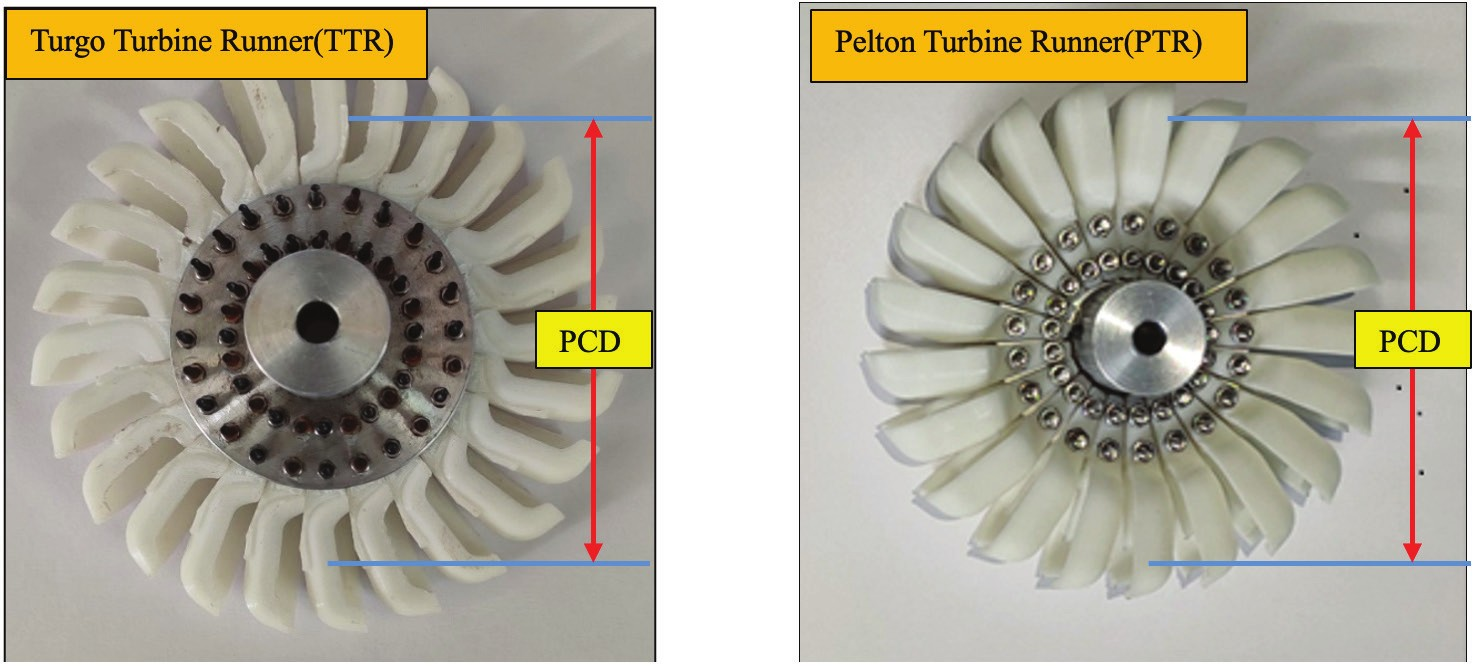
\includegraphics[width=0.85\textwidth]{Articulo_LaTeX/Figs/lakdawala_rodetes.jpg}
\caption{Las dos turbinas del experimento, Turgo (izquierda) y Pelton (derecha), vistas desde arriba. La flecha roja marca el diámetro de la circunferencia donde el chorro golpea los cangilones, que es el mismo en las dos. Fuente: (Lakdawala, 2025).}
\label{fig:rodetes}
\end{figure}

Las turbinas se probaron en el banco de pruebas de la Figura~\ref{fig:montaje}, con la misma altura de agua en todos los ensayos. Una bomba lleva el agua hasta las boquillas, el chorro hace girar la rueda y, en cada ensayo, se midieron el caudal de agua, la velocidad de giro de la rueda y la fuerza de giro en el eje; con esas tres mediciones se calculó la eficiencia. Los detalles técnicos del montaje no son necesarios para el análisis estadístico, pero los términos que aparecen en el artículo original se explican en el glosario del Apéndice~\ref{sec:glosario}.

\begin{figure}[H]
\centering
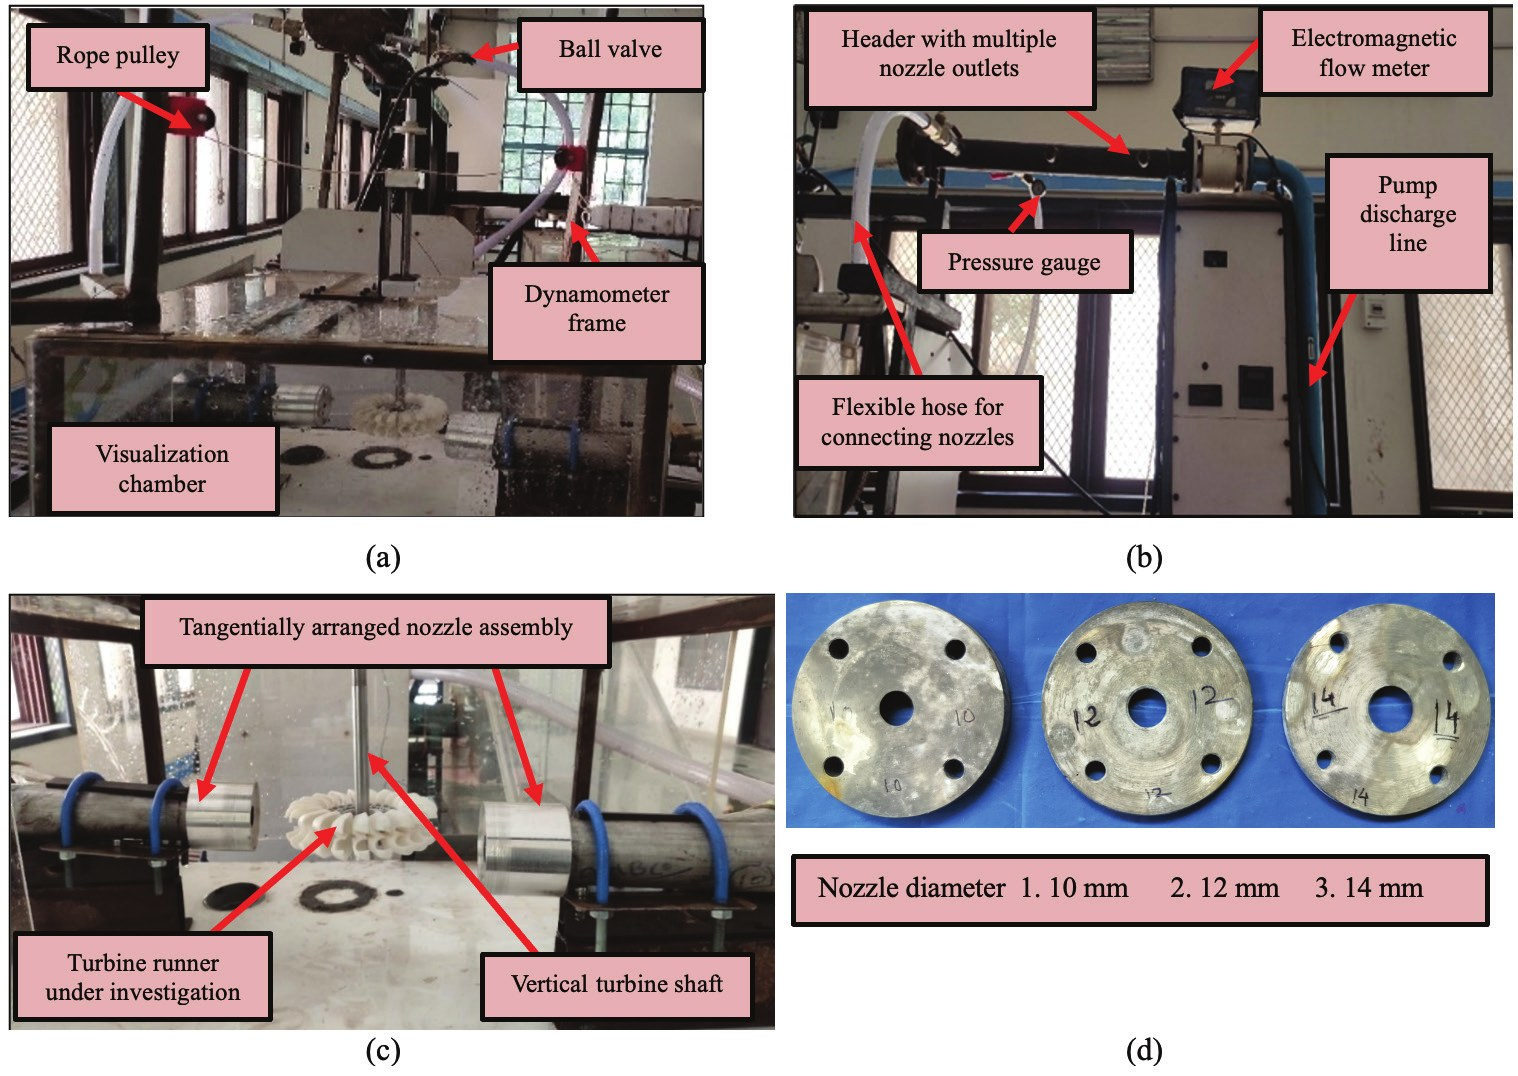
\includegraphics[width=0.9\textwidth]{Articulo_LaTeX/Figs/lakdawala_montaje.jpg}
\caption{Banco de pruebas: (a) sistema para medir la fuerza de giro en el eje, (b) tubería con el medidor de caudal, (c) las dos boquillas frente a la turbina y (d) las tres placas que fijan el diámetro de la boquilla (10, 12 y 14~mm). Fuente: (Lakdawala, 2025).}
\label{fig:montaje}
\end{figure}

En cada uno de los 80 ensayos, llamados corridas, los investigadores fijaron cinco variables: el tipo de turbina (Pelton o Turgo), el número de boquillas (una o dos) y tres características de la boquilla, que son su diámetro (10, 12 o 14~mm), su ángulo y su distancia a la rueda. La Figura~\ref{fig:chorro} muestra qué significan las dos últimas. El ángulo indica qué tan de frente llega el chorro a la rueda: 90° es perpendicular y 92.5° y 95° son desviaciones pequeñas. La distancia es el recorrido del chorro entre la boquilla y la rueda, que se varió entre 40 y 60~mm.

\begin{figure}[H]
\centering
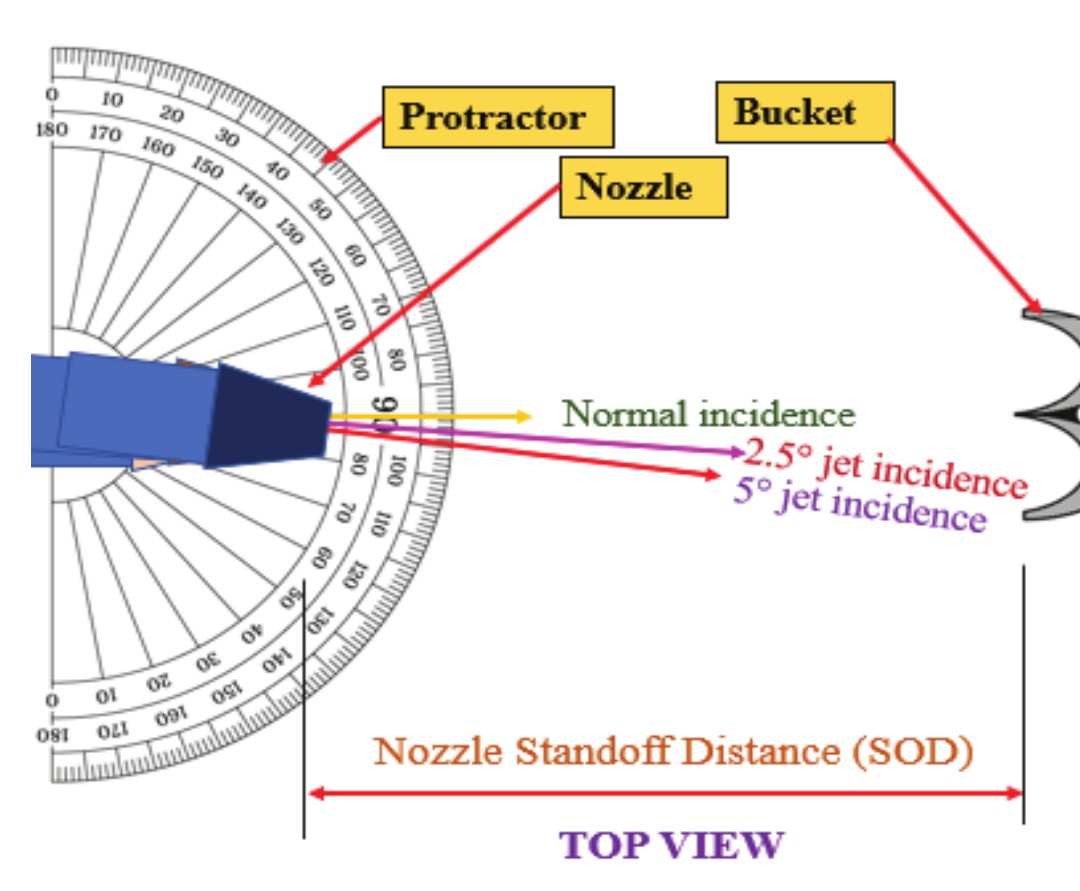
\includegraphics[width=0.55\textwidth]{Articulo_LaTeX/Figs/lakdawala_chorro.jpg}
\caption{Vista desde arriba de la boquilla y un cangilón: ángulo del chorro (perpendicular, desviado 2.5° y desviado 5°) y distancia entre la boquilla y el cangilón (\textit{Nozzle Standoff Distance}). Fuente: (Lakdawala, 2025).}
\label{fig:chorro}
\end{figure}

Las combinaciones de valores no se escogieron al azar. Los autores usaron un diseño central compuesto, un tipo de diseño experimental pensado para ajustar modelos de regresión con términos cuadráticos usando pocas corridas. Por eso cada variable numérica toma solo tres valores (bajo, medio y alto) y varias corridas se repiten en el punto central, con las tres variables en su valor medio. Con estos datos, los autores ajustaron un modelo de regresión cuadrático y buscaron la combinación de variables que maximiza la eficiencia.

En este trabajo se usan los datos publicados por (Lakdawala, 2025) para estudiar, con las herramientas del análisis de regresión, cómo se relaciona la eficiencia hidráulica con las cinco variables. Esta parte presenta la descripción de los datos y el análisis exploratorio, que orientan la construcción del modelo. Todos los cálculos y gráficos se hicieron en R con los paquetes \textsf{ggplot2} y \textsf{GGally}, y el código está en el repositorio indicado en la sección de disponibilidad de datos.


\section{Metodología}
\label{sec:metodologia}
\subsection{Datos}
\label{sec:datos}

Los datos provienen de la Tabla~6 de Lakdawala (2025) y corresponden a las 80 corridas descritas en la introducción. La variable respuesta es la eficiencia hidráulica, expresada como proporción (entre 0 y 1). La Tabla~\ref{tab:variables} resume las variables y el nombre con el que aparecen en la base de datos.

\begin{table}[H]
\centering
\caption{Variables del estudio.}
\label{tab:variables}
\begin{tabular}{llll}
\toprule
Variable & Nombre en R & Tipo & Niveles \\
\midrule
Eficiencia hidráulica ($y$)            & \texttt{eficiencia} & Respuesta numérica   & 0.6025 a 0.7165 \\
Ángulo de la boquilla ($\alpha$)       & \texttt{angulo}     & Numérica (grados)    & 90, 92.5, 95 \\
Diámetro de la boquilla ($d_j$)        & \texttt{diametro}   & Numérica (mm)        & 10, 12, 14 \\
Distancia boquilla-rodete ($N_{sod}$)  & \texttt{distancia}  & Numérica (mm)        & 40, 50, 60 \\
Tipo de rodete                         & \texttt{rodete}     & Categórica           & Pelton (PTR), Turgo (TTR) \\
Número de boquillas ($n$)              & \texttt{boquillas}  & Categórica           & 1, 2 \\
\bottomrule
\end{tabular}
\end{table}

Los datos y el código del análisis están disponibles en \enlacerepositorio. El script \texttt{anal\_descrip.R} lee los datos desde el repositorio y produce todas las tablas, cifras y figuras de la Sección~\ref{sec:resultados}.


\section{Resultados}
\label{sec:resultados}
\subsection{Análisis descriptivo}
\label{sec:descriptivo}

\subsubsection{Distribución de la eficiencia hidráulica}

La Tabla~\ref{tab:resumen_y} resume la eficiencia hidráulica de las 80 corridas (sección~4 del script). La eficiencia media es de 0.6540, con una desviación estándar de 0.0245 y un coeficiente de variación de 3.74\,\%, es decir, las eficiencias cambian poco en términos relativos. Los valores van de 0.6025 a 0.7165.

Además de la media y la desviación estándar, la tabla incluye tres medidas de la forma de la distribución:

\begin{itemize}[leftmargin=*, itemsep=2pt]
  \item \textbf{Rango intercuartílico (RIQ).} Es la diferencia entre el tercer cuartil ($Q_3$, el valor que deja por debajo al 75\,\% de los datos) y el primer cuartil ($Q_1$, que deja por debajo al 25\,\%): $\text{RIQ} = Q_3 - Q_1$. Mide la amplitud del 50\,\% central de los datos y, a diferencia del rango o la desviación estándar, no se ve afectado por valores extremos. Aquí $Q_1 = 0.6360$ y $Q_3 = 0.6715$, así que la mitad central de las corridas tiene eficiencias en un intervalo de apenas 0.0355.

  \item \textbf{Asimetría.} Mide si la distribución se extiende más hacia un lado que hacia el otro. Se calcula como
  \[
  g_1 = \frac{\frac{1}{n}\sum_{i=1}^{n}(y_i-\bar{y})^3}{s^3}.
  \]
  Vale cero en una distribución simétrica, es positiva cuando la cola derecha es más larga (hay algunos valores altos alejados del resto) y negativa cuando la cola larga está a la izquierda. El valor de 0.380 indica una asimetría leve hacia la derecha: hay algunas corridas con eficiencias altas, cercanas a 0.70, más alejadas de la media que las corridas de eficiencia baja. Por eso la media (0.6540) queda un poco por encima de la mediana (0.6515).

  \item \textbf{Exceso de curtosis.} La curtosis mide qué tan pesadas son las colas de una distribución, es decir, qué tanto pesan los valores muy alejados de la media. Se calcula como $\frac{1}{n}\sum_{i=1}^{n}(y_i-\bar{y})^4 / s^4$, y en una distribución normal vale 3. Por eso se suele reportar el \emph{exceso} de curtosis, que es la curtosis menos 3, de modo que la normal sirva de referencia con un valor de cero. Un exceso positivo indica colas más pesadas que la normal (más valores extremos de lo esperado) y uno negativo, colas más livianas. El valor de $-0.351$ indica que las eficiencias tienen colas algo más livianas que una normal: hay pocos valores muy alejados de la media.
\end{itemize}

\begin{table}[H]
\centering
\caption{Medidas descriptivas de la eficiencia hidráulica ($n = 80$).}
\label{tab:resumen_y}
\begin{tabular}{lc@{\hspace{1.5cm}}lc}
\toprule
Medida & Valor & Medida & Valor \\
\midrule
Media               & 0.6540 & Mínimo                  & 0.6025 \\
Mediana             & 0.6515 & Máximo                  & 0.7165 \\
Desviación estándar & 0.0245 & Rango intercuartílico   & 0.0355 \\
Coef. de variación  & 3.74\,\% & Asimetría             & 0.380 \\
                    &        & Exceso de curtosis      & $-0.351$ \\
\bottomrule
\end{tabular}
\end{table}

La Figura~\ref{fig:distribucion} muestra estas características de forma gráfica. El panel~(a) es un histograma: el rango de eficiencias se divide en 12 intervalos y la altura de cada barra indica cuántas corridas caen en ese intervalo, en escala de densidad (el área total de las barras suma uno). La curva negra es una estimación suavizada de esa densidad y la línea roja discontinua marca la media. Se ve una distribución con un solo pico, alrededor de 0.65, y una cola derecha un poco más larga, lo que coincide con la asimetría positiva.

El panel~(b) es un diagrama de caja. La caja va del primer al tercer cuartil ($Q_1 = 0.6360$ y $Q_3 = 0.6715$), así que su altura es el rango intercuartílico y contiene al 50\,\% central de las corridas; la línea negra dentro de la caja es la mediana. Los bigotes se extienden hasta la corrida más extrema que esté a menos de $1.5 \times \text{RIQ}$ de la caja, es decir, entre 0.5828 y 0.7248; los valores por fuera de esos límites se considerarían atípicos. Los puntos negros son las 80 corridas, separadas un poco en horizontal para que no se superpongan. Ninguna corrida queda por fuera de los bigotes, así que no hay eficiencias atípicas, y la mediana está algo más cerca del borde inferior de la caja, otra señal de la leve asimetría a la derecha.

\begin{figure}[H]
\centering
\begin{minipage}[b]{0.62\textwidth}
  \centering
  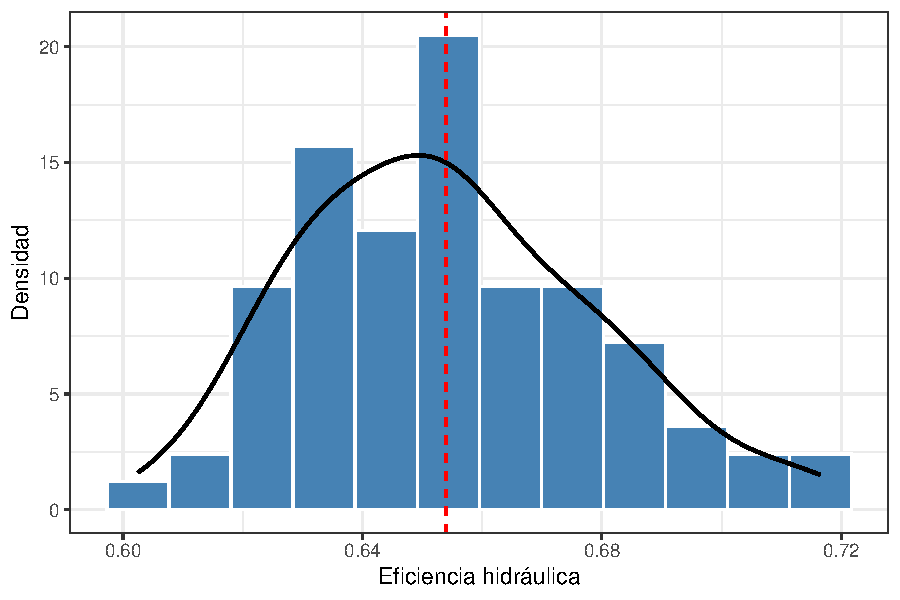
\includegraphics[width=\textwidth]{Articulo_LaTeX/Figs/g1_histograma.pdf}\\[-2pt]
  {\small (a)}
\end{minipage}\hfill
\begin{minipage}[b]{0.35\textwidth}
  \centering
  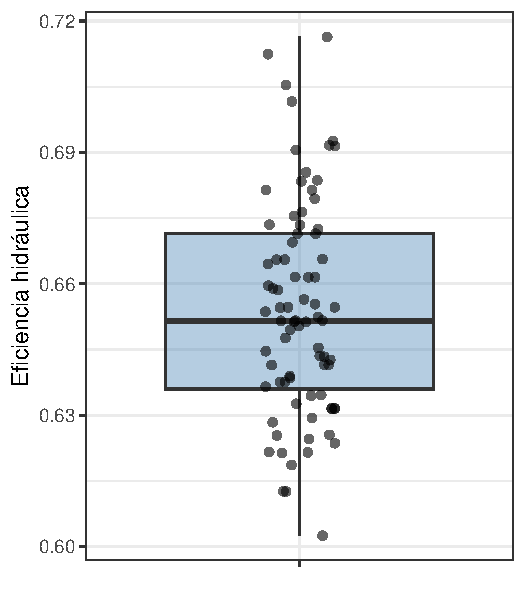
\includegraphics[width=\textwidth]{Articulo_LaTeX/Figs/g2_boxplot.pdf}\\[-2pt]
  {\small (b)}
\end{minipage}
\caption{Histograma con curva de densidad (a) y diagrama de caja (b) de la eficiencia hidráulica. La línea roja discontinua marca la media. Código: sección~4 de \texttt{anal\_descrip.R}.}
\label{fig:distribucion}
\end{figure}

\subsubsection{Eficiencia según cada variable explicativa}

La Tabla~\ref{tab:niveles} y la Figura~\ref{fig:por_variable} muestran la eficiencia según cada variable explicativa (sección~5 del script). En la figura hay un diagrama de caja por cada nivel de cada variable, construido igual que en la Figura~\ref{fig:distribucion}(b) pero solo con las corridas de ese nivel; los puntos azules son las corridas y el rombo rojo es la media del grupo. Si las cajas de los distintos niveles están a alturas diferentes, la variable está asociada con la eficiencia; si se superponen mucho, la diferencia entre niveles es pequeña comparada con la variación dentro de cada nivel. Los niveles medios (92.5°, 12~mm y 50~mm) tienen el doble de corridas que los extremos porque ahí están las réplicas del punto central.

\begin{table}[H]
\centering
\caption{Eficiencia hidráulica según el nivel de cada variable explicativa.}
\label{tab:niveles}
\begin{tabular}{llccccc}
\toprule
Variable & Nivel & $n$ & Media & Desv. est. & Mínimo & Máximo \\
\midrule
\multirow{3}{*}{Ángulo (°)}       & 90    & 21 & 0.6788 & 0.0219 & 0.6285 & 0.7165 \\
                                  & 92.5  & 40 & 0.6478 & 0.0171 & 0.6185 & 0.6915 \\
                                  & 95    & 19 & 0.6394 & 0.0208 & 0.6025 & 0.6835 \\
\midrule
\multirow{3}{*}{Diámetro (mm)}    & 10    & 20 & 0.6618 & 0.0271 & 0.6125 & 0.7165 \\
                                  & 12    & 40 & 0.6507 & 0.0193 & 0.6215 & 0.7055 \\
                                  & 14    & 20 & 0.6527 & 0.0300 & 0.6025 & 0.7125 \\
\midrule
\multirow{3}{*}{Distancia (mm)}   & 40    & 21 & 0.6679 & 0.0260 & 0.6255 & 0.7165 \\
                                  & 50    & 40 & 0.6492 & 0.0188 & 0.6185 & 0.7055 \\
                                  & 60    & 19 & 0.6485 & 0.0282 & 0.6025 & 0.7015 \\
\midrule
\multirow{2}{*}{Rodete}           & Pelton & 40 & 0.6441 & 0.0212 & 0.6025 & 0.6925 \\
                                  & Turgo  & 40 & 0.6638 & 0.0238 & 0.6125 & 0.7165 \\
\midrule
\multirow{2}{*}{Boquillas}        & 1     & 40 & 0.6429 & 0.0211 & 0.6025 & 0.6915 \\
                                  & 2     & 40 & 0.6650 & 0.0227 & 0.6235 & 0.7165 \\
\bottomrule
\end{tabular}
\end{table}

El ángulo de la boquilla es la variable con el efecto más claro: la eficiencia media baja de 0.679 a 90° a 0.639 a 95°, y la caja de 90° está casi por completo por encima de las otras dos. El rodete Turgo es en promedio más eficiente que el Pelton (0.664 frente a 0.644) y usar dos boquillas también aumenta la eficiencia media (0.665 frente a 0.643); en ambos casos las cajas se desplazan hacia arriba, aunque se superponen en parte. Con el diámetro y la distancia la eficiencia media es mayor en el nivel bajo (10~mm y 40~mm), pero las diferencias son menores y las cajas se superponen mucho, porque la dispersión dentro de cada nivel es grande.

\begin{figure}[H]
\centering

\includegraphics[width=0.92\textwidth]{Articulo_LaTeX/Figs/g3_boxplot_por_variable.pdf}
\caption{Eficiencia hidráulica según cada variable explicativa. Los rombos rojos marcan la media de cada grupo. Código: sección~5 de \texttt{anal\_descrip.R}.}
\label{fig:por_variable}
\end{figure}

\subsubsection{Eficiencia media con intervalos de confianza}

Los diagramas de caja muestran cómo se reparten las corridas; para comparar los niveles conviene mirar también qué tan precisa es cada media. La Figura~\ref{fig:medias} muestra la eficiencia media de cada nivel con su intervalo de confianza del 95\,\%, calculado con la distribución $t$ de Student:
\[
\bar{y} \pm t_{0.975,\,n-1}\,\frac{s}{\sqrt{n}},
\]
donde $\bar{y}$, $s$ y $n$ son la media, la desviación estándar y el número de corridas del nivel. Cada punto es una media, las barras son el intervalo y la línea une las medias para mostrar la tendencia. La Tabla~\ref{tab:ic} presenta los mismos intervalos (sección~6 del script).

\begin{figure}[H]
\centering
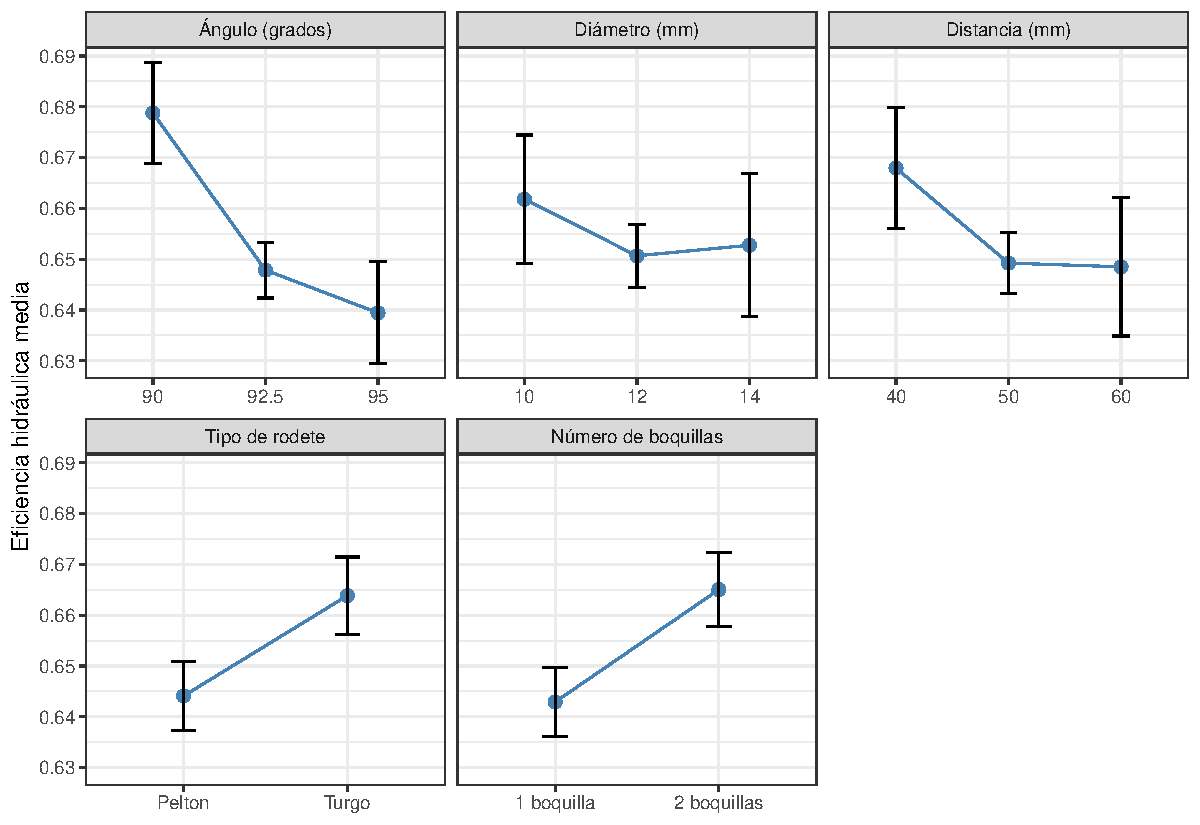
\includegraphics[width=0.92\textwidth]{Articulo_LaTeX/Figs/g4_medias_ic95.pdf}
\caption{Eficiencia media e intervalo de confianza del 95\,\% para cada nivel de cada variable explicativa. Código: sección~6 de \texttt{anal\_descrip.R}.}
\label{fig:medias}
\end{figure}

\begin{table}[H]
\centering
\caption{Eficiencia media e intervalo de confianza del 95\,\% por nivel.}
\label{tab:ic}
\begin{tabular}{llcccc}
\toprule
Variable & Nivel & Media & Límite inferior & Límite superior & Ancho \\
\midrule
\multirow{3}{*}{Ángulo (°)}     & 90     & 0.6788 & 0.6688 & 0.6888 & 0.0200 \\
                                & 92.5   & 0.6478 & 0.6424 & 0.6533 & 0.0109 \\
                                & 95     & 0.6394 & 0.6294 & 0.6495 & 0.0201 \\
\midrule
\multirow{3}{*}{Diámetro (mm)}  & 10     & 0.6618 & 0.6491 & 0.6745 & 0.0254 \\
                                & 12     & 0.6507 & 0.6445 & 0.6569 & 0.0124 \\
                                & 14     & 0.6527 & 0.6387 & 0.6668 & 0.0281 \\
\midrule
\multirow{3}{*}{Distancia (mm)} & 40     & 0.6679 & 0.6561 & 0.6798 & 0.0237 \\
                                & 50     & 0.6492 & 0.6432 & 0.6553 & 0.0121 \\
                                & 60     & 0.6485 & 0.6349 & 0.6621 & 0.0272 \\
\midrule
\multirow{2}{*}{Rodete}         & Pelton & 0.6441 & 0.6373 & 0.6509 & 0.0136 \\
                                & Turgo  & 0.6638 & 0.6562 & 0.6714 & 0.0152 \\
\midrule
\multirow{2}{*}{Boquillas}      & 1      & 0.6429 & 0.6362 & 0.6497 & 0.0135 \\
                                & 2      & 0.6650 & 0.6578 & 0.6723 & 0.0145 \\
\bottomrule
\end{tabular}
\end{table}

Una forma informal de leer la figura es fijarse si los intervalos de dos niveles se superponen. Con el ángulo, el intervalo de 90° $[0.6688;\ 0.6888]$ queda completamente por encima de los de 92.5° y 95°, mientras que estos dos últimos se superponen, así que la caída fuerte ocurre entre 90° y 92.5°. Con el tipo de rodete y el número de boquillas los intervalos no se superponen: el Turgo y el uso de dos boquillas tienen una eficiencia media claramente mayor. Con la distancia, el intervalo de 40~mm apenas queda por encima del de 50~mm (0.6561 frente a 0.6553) y se superpone con el de 60~mm. Con el diámetro, los tres intervalos se superponen, de modo que estos datos no muestran por sí solos una diferencia clara entre diámetros.

Los intervalos de los niveles medios son más angostos (alrededor de 0.011 a 0.012, frente a 0.020 a 0.028 en los extremos) porque tienen el doble de corridas y el ancho del intervalo decrece con $\sqrt{n}$. Hay que tener en cuenta dos cosas al interpretar esta figura. Primero, cada media promedia sobre todos los valores de las demás variables, así que no aísla el efecto de una variable manteniendo las otras fijas; eso lo hace el modelo de regresión. Segundo, que dos intervalos se superpongan no prueba que las medias sean iguales: es solo una guía visual, y la comparación formal se hará con las pruebas del modelo.

\subsubsection{Posibles interacciones}

La Figura~\ref{fig:perfiles} presenta gráficos de perfiles (sección~7 del script). Cada línea corresponde a una combinación de tipo de rodete y número de boquillas, y cada punto es la eficiencia media de las corridas de esa combinación en un nivel de la variable del eje horizontal. Este gráfico sirve para buscar interacciones: si el efecto de una variable es el mismo en todas las combinaciones, las líneas son paralelas y solo se desplazan hacia arriba o hacia abajo; si las líneas tienen pendientes distintas o se cruzan, el efecto de esa variable depende del tipo de rodete o del número de boquillas.

\begin{figure}[H]
\centering
\begin{minipage}[b]{0.49\textwidth}
  \centering
  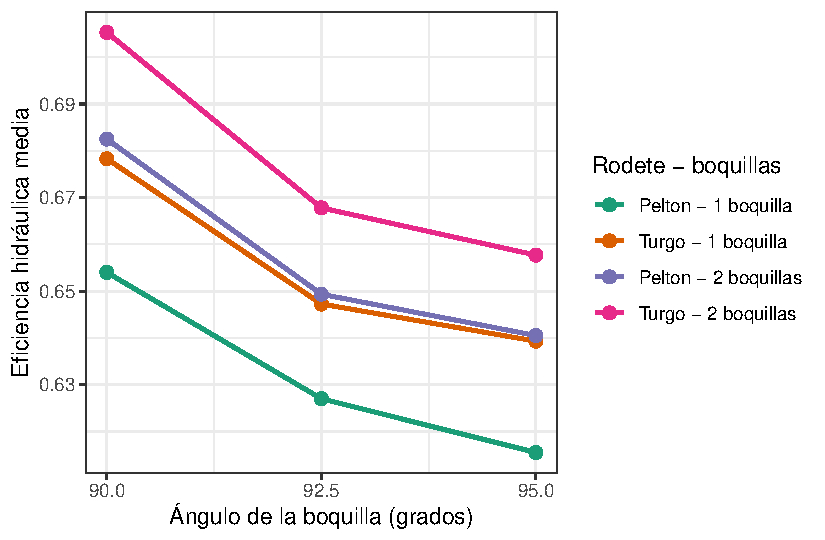
\includegraphics[width=\textwidth]{Articulo_LaTeX/Figs/perfil_angulo.pdf}\\[-2pt]
  {\small (a)}
\end{minipage}\hfill
\begin{minipage}[b]{0.49\textwidth}
  \centering
  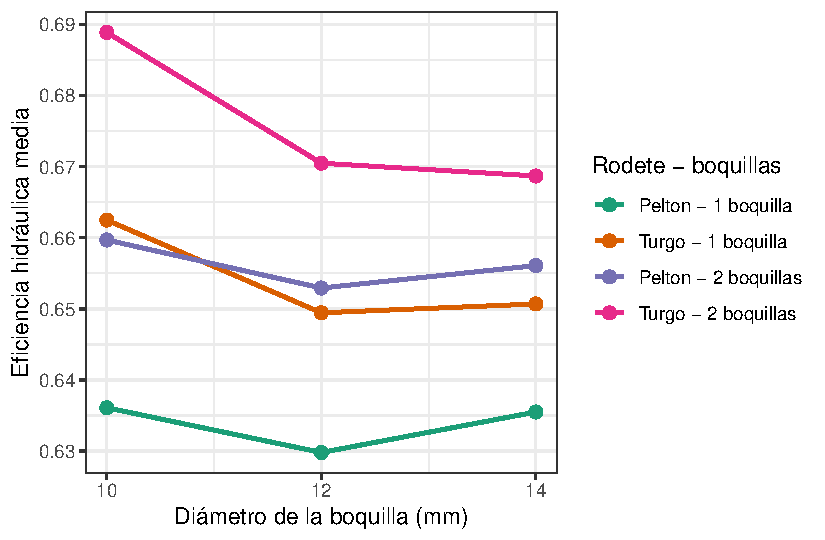
\includegraphics[width=\textwidth]{Articulo_LaTeX/Figs/perfil_diametro.pdf}\\[-2pt]
  {\small (b)}
\end{minipage}\\[6pt]
\begin{minipage}[b]{0.49\textwidth}
  \centering
  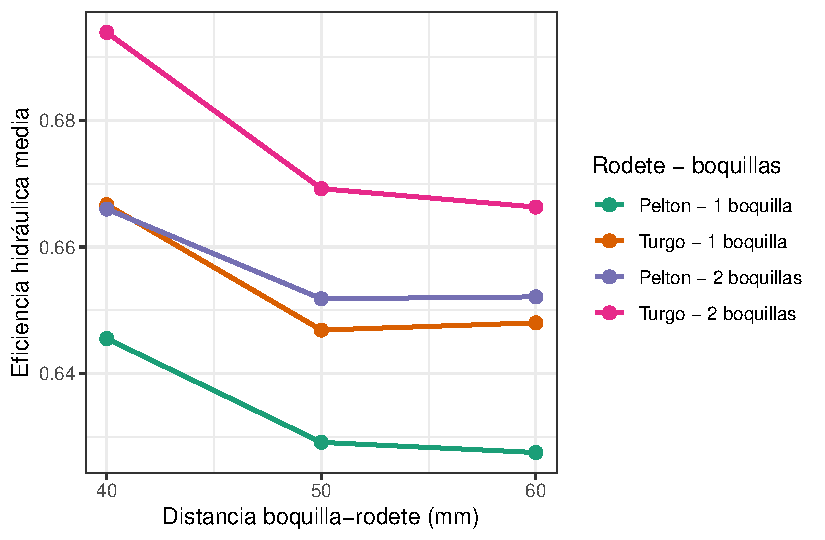
\includegraphics[width=\textwidth]{Articulo_LaTeX/Figs/perfil_distancia.pdf}\\[-2pt]
  {\small (c)}
\end{minipage}
\caption{Perfiles de la eficiencia media según el ángulo (a), el diámetro (b) y la distancia (c), para cada combinación de tipo de rodete y número de boquillas. Código: sección~7 de \texttt{anal\_descrip.R}.}
\label{fig:perfiles}
\end{figure}

Se ven tres cosas. Primero, la separación vertical entre las líneas confirma los efectos del tipo de rodete y del número de boquillas: el Turgo con dos boquillas va siempre por encima (por ejemplo, 0.7053 a 90°) y el Pelton con una boquilla siempre por debajo (0.6540 a 90°), mientras que el Turgo con una boquilla y el Pelton con dos quedan casi superpuestos en la mitad. Segundo, con el ángulo y con la distancia la eficiencia cae más del nivel bajo al nivel medio que del nivel medio al alto (en el Pelton con una boquilla, por ejemplo, pasa de 0.6540 a 0.6270 y luego a 0.6155 con el ángulo), lo que sugiere curvatura y justifica probar términos cuadráticos. Tercero, las líneas son aproximadamente paralelas, aunque con algunas diferencias de forma: con el diámetro, el Turgo con dos boquillas baja de 0.6889 a 0.6705 entre 10 y 12~mm, mientras que el Pelton con dos boquillas solo baja de 0.6597 a 0.6529. El ajuste del modelo dirá si esas diferencias corresponden a interacciones significativas.

\subsubsection{Gráfico condicional}

La Figura~\ref{fig:condicional} muestra cada corrida por separado (sección~8 del script). El eje horizontal es el ángulo y el vertical la eficiencia; los cuatro paneles separan el tipo de rodete (columnas) y el número de boquillas (filas), y el color indica el diámetro de la boquilla. Los puntos se movieron un poco en horizontal para que no se tapen entre sí. A diferencia de los gráficos anteriores, que resumen con medias, este permite ver tres variables a la vez sin promediar.

\begin{figure}[H]
\centering
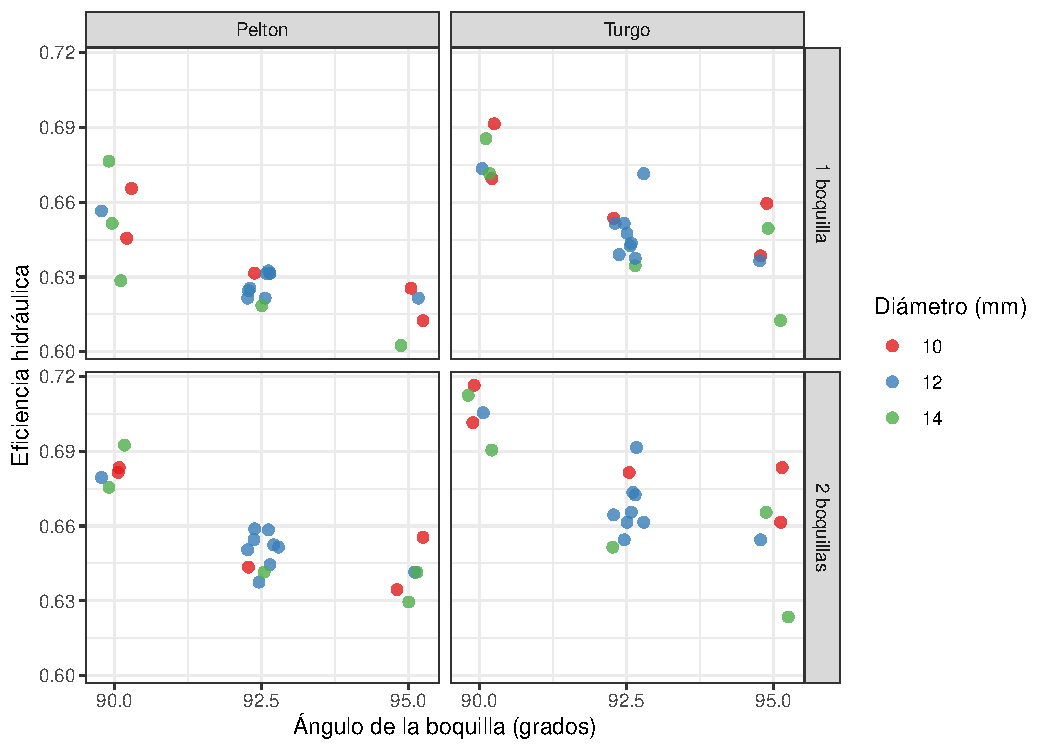
\includegraphics[width=0.85\textwidth]{Articulo_LaTeX/Figs/g5_condicional.pdf}
\caption{Eficiencia frente al ángulo de la boquilla, por tipo de rodete (columnas) y número de boquillas (filas); el color indica el diámetro. Código: sección~8 de \texttt{anal\_descrip.R}.}
\label{fig:condicional}
\end{figure}

En los cuatro paneles la eficiencia baja al pasar de 90° a 95°, así que el efecto del ángulo se repite en todas las combinaciones de rodete y número de boquillas. Los paneles de la derecha (Turgo) y los de abajo (dos boquillas) están en general más arriba, lo que coincide con lo visto en las medias. El color aporta algo nuevo: con 95° los puntos verdes (14~mm) quedan casi siempre entre los más bajos de cada panel, mientras que con 90° los tres colores están mezclados. La Tabla~\ref{tab:angulo_diametro} lo resume con las medias: con 90° la eficiencia media con 14~mm es solo 0.0058 menor que con 10~mm, pero con 95° la diferencia es de 0.0143. Es decir, el efecto del diámetro parece depender del ángulo, lo que sugiere una posible interacción entre estas dos variables.

\begin{table}[H]
\centering
\caption{Eficiencia media según el ángulo y el diámetro de la boquilla.}
\label{tab:angulo_diametro}
\begin{tabular}{lccc}
\toprule
 & \multicolumn{3}{c}{Diámetro (mm)} \\
\cmidrule(lr){2-4}
Ángulo (°) & 10 & 12 & 14 \\
\midrule
90   & 0.6819 & 0.6788 & 0.6761 \\
92.5 & 0.6525 & 0.6487 & 0.6365 \\
95   & 0.6464 & 0.6385 & 0.6321 \\
\bottomrule
\end{tabular}
\end{table}

\subsubsection{Correlaciones y matriz de dispersión}

La Tabla~\ref{tab:correlaciones} presenta las correlaciones entre la eficiencia y las variables numéricas (sección~9 del script). La correlación de Pearson mide la fuerza de la relación lineal; la de Spearman se calcula sobre los rangos de los datos y mide si la relación es monótona (siempre creciente o siempre decreciente), aunque no sea una recta. Las tres relaciones son negativas y la del ángulo es la más fuerte, lo que coincide con lo visto en las figuras anteriores. Los dos coeficientes son muy parecidos en las tres variables, lo que indica que las relaciones son monótonas y que no hay valores extremos que distorsionen la correlación de Pearson.

\begin{table}[H]
\centering
\caption{Correlación de la eficiencia con las variables numéricas.}
\label{tab:correlaciones}
\begin{tabular}{lcc}
\toprule
Variable & Pearson & Spearman \\
\midrule
Ángulo    & $-0.580$ & $-0.552$ \\
Diámetro  & $-0.132$ & $-0.137$ \\
Distancia & $-0.289$ & $-0.273$ \\
\bottomrule
\end{tabular}
\end{table}

La Figura~\ref{fig:matriz} es una matriz de dispersión que reúne todas las variables en un solo gráfico, con el Pelton en verde y el Turgo en naranja. Se lee así:
\begin{itemize}[leftmargin=*, itemsep=2pt]
  \item \textbf{Debajo de la diagonal} están los diagramas de dispersión de cada par de variables. Entre las explicativas los puntos forman una cuadrícula, porque cada una toma solo tres valores fijados por el diseño.
  \item \textbf{En la diagonal} está la densidad de cada variable para cada tipo de rodete. Las de las explicativas son prácticamente iguales en los dos rodetes, porque ambos se probaron con el mismo diseño; la de la eficiencia del Turgo está corrida hacia la derecha.
  \item \textbf{Encima de la diagonal} está la correlación de cada par, primero para todos los datos (\textit{Corr}) y luego dentro de cada rodete. Los asteriscos indican si la correlación es significativamente distinta de cero: *** para $p < 0.001$, ** para $p < 0.01$, * para $p < 0.05$ y un punto para $p < 0.1$.
  \item \textbf{La última columna} compara cada variable entre los dos rodetes con diagramas de caja, y \textbf{la última fila} muestra los histogramas por rodete.
\end{itemize}

\begin{figure}[H]
\centering
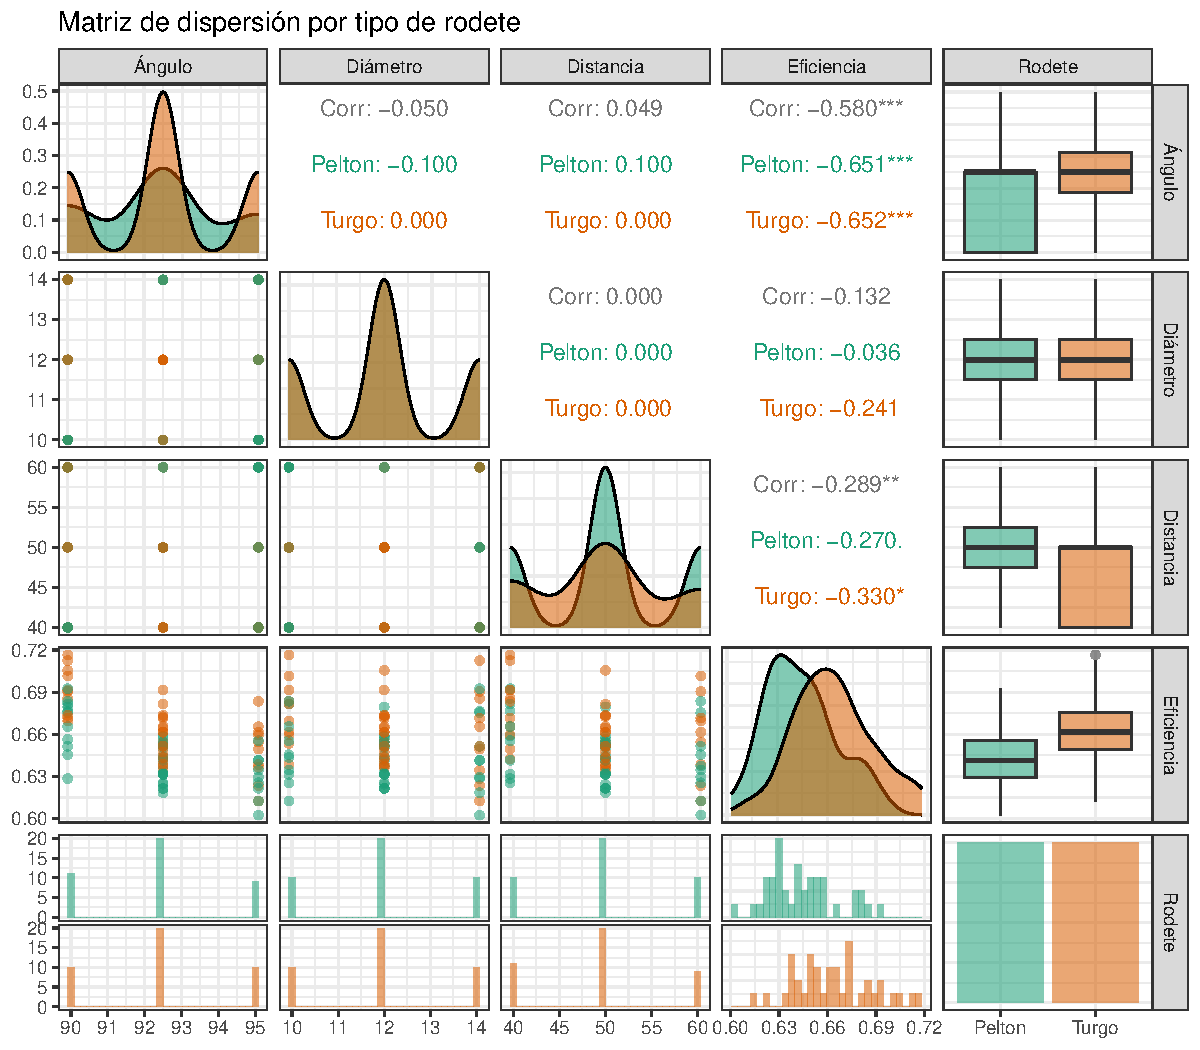
\includegraphics[width=0.9\textwidth]{Articulo_LaTeX/Figs/g6_matriz_dispersion.pdf}
\caption{Matriz de dispersión de las variables numéricas y del tipo de rodete (verde: Pelton, naranja: Turgo). Código: sección~9 de \texttt{anal\_descrip.R}.}
\label{fig:matriz}
\end{figure}

La información nueva está en las correlaciones dentro de cada rodete. La del ángulo con la eficiencia es de $-0.651$ en el Pelton y $-0.652$ en el Turgo, más fuerte que la total ($-0.580$): al juntar los dos rodetes, la diferencia de nivel entre ellos agrega variación que no tiene que ver con el ángulo y debilita la correlación. La del diámetro es casi nula en el Pelton ($-0.036$) pero de $-0.241$ en el Turgo, y la de la distancia es de $-0.270$ en el Pelton y $-0.330$ en el Turgo. Que la relación del diámetro con la eficiencia cambie según el rodete es otra señal de una posible interacción, en este caso entre el diámetro y el tipo de rodete.

Por último, entre las propias variables explicativas las correlaciones son prácticamente nulas (en valor absoluto, 0.1 o menos), tanto con todos los datos como dentro de cada rodete. Es lo que se espera en un diseño experimental, donde los investigadores fijan los valores de cada variable de forma planificada y no dejan que cambien juntas.


% \section{Análisis de resultados}
% \label{sec:analisis}
% \subsection{Comparación con el artículo original}

Lakdawala (2025) ajustaron el modelo cuadrático~\eqref{eq:cuadratico} con el programa Design Expert y reportaron un modelo significativo ($F = 90.49$, $p < 0.0001$), sin evidencia de falta de ajuste ($F = 0.97$, $p = 0.5454$). Según su tabla ANOVA, los términos significativos al 5\,\% fueron los cinco efectos principales, las interacciones ángulo $\times$ diámetro, ángulo $\times$ distancia, diámetro $\times$ distancia, diámetro $\times$ rodete y distancia $\times$ rodete, y los términos cuadráticos del ángulo y de la distancia. La Tabla~\ref{tab:anova_original} resume esos resultados como referencia para comparar.

\begin{table}[H]
\centering
\caption{Resumen de la tabla ANOVA reportada por Lakdawala (2025) para el modelo cuadrático.}
\label{tab:anova_original}
\begin{tabular}{lccc}
\toprule
Término & $F$ & Valor $p$ & ¿Significativo al 5\,\%? \\
\midrule
Ángulo ($\alpha$)                 & 642.26 & $<0.0001$ & Sí \\
Diámetro ($d_j$)                  & 29.26  & $<0.0001$ & Sí \\
Distancia ($N_{sod}$)             & 157.85 & $<0.0001$ & Sí \\
Tipo de rodete                    & 278.07 & $<0.0001$ & Sí \\
Número de boquillas               & 349.69 & $<0.0001$ & Sí \\
Ángulo $\times$ diámetro          & 15.81  & 0.0002    & Sí \\
Ángulo $\times$ distancia         & 4.15   & 0.0459    & Sí \\
Diámetro $\times$ distancia       & 4.43   & 0.0394    & Sí \\
Diámetro $\times$ rodete          & 17.26  & 0.0001    & Sí \\
Distancia $\times$ rodete         & 9.22   & 0.0035    & Sí \\
Ángulo$^2$                        & 50.33  & $<0.0001$ & Sí \\
Distancia$^2$                     & 7.49   & 0.0081    & Sí \\
Diámetro$^2$                      & 3.10   & 0.0834    & No \\
Diámetro $\times$ boquillas       & 2.90   & 0.0936    & No \\
Ángulo $\times$ boquillas         & 2.06   & 0.1565    & No \\
Ángulo $\times$ rodete            & 0.29   & 0.5926    & No \\
Rodete $\times$ boquillas         & 0.18   & 0.6756    & No \\
Distancia $\times$ boquillas      & 0.03   & 0.8676    & No \\
\midrule
Falta de ajuste                   & 0.97   & 0.5454    & No \\
\bottomrule
\end{tabular}
\end{table}

\pendiente{Comparar estos resultados con los de tu modelo: ¿se repiten los términos significativos?, ¿cambian las conclusiones al revisar supuestos y puntos influyentes?}

%
% \section{Conclusiones}
% \label{sec:conclusiones}

\FloatBarrier
\subsection*{Disponibilidad de datos y código}

Los datos y el código en R usados en este trabajo están disponibles en el repositorio \enlacerepositorio.
  

% ---------------- Referencias ---------------------

\section{Referencias bibliográficas}

Lakdawala, H. N. (2025). Performance optimization of low-head vertical axis impulse turbine runners for nozzle angle, nozzle diameter, and nozzle standoff distance using response surface methodology. \textit{Journal Of Thermal Engineering}, 1392-1419. \url{https://doi.org/10.14744/thermal.0000983}

El artículo se encuentra disponible en:

\url{https://drive.google.com/file/d/11gxh1VBlpA0WJfVSf1WYcSbQmxDbRhIN/view?usp=sharing}

% ---------------- Apéndices -----------------------
\appendix
\section{Glosario}
\label{sec:glosario}
% ---------------------------------------------------
% Glosario de términos usados en Lakdawala et al. (2025)
% Formato: \item[Término] (\textit{término en inglés}) definición
% ---------------------------------------------------

Este glosario reúne los términos técnicos que aparecen en Lakdawala (2025). Entre paréntesis se indica el término en inglés usado en el artículo y, cuando aplica, su notación.

\subsection*{Turbinas y banco de pruebas}

\begin{description}[style=nextline, leftmargin=1.2em, itemsep=3pt, font=\normalfont\bfseries\color{verdeOscuroUN}]

\item[Pico central hidroeléctrica] (\textit{pico hydro}) Instalación hidroeléctrica de muy pequeña potencia, pensada para abastecer cargas aisladas, fuera de la red eléctrica (\textit{off-grid}). El prefijo \textit{pico} se refiere al rango de potencia del generador.

\item[Turbina de impulso] (\textit{impulse turbine}) Turbina en la que el agua sale de una boquilla convertida en un chorro de alta velocidad y transmite su energía cinética al rodete al golpear los cangilones, a presión atmosférica. Las turbinas Pelton y Turgo son de este tipo.

\item[Turbina Pelton] (\textit{Pelton Turbine Runner}, PTR) Turbina de impulso cuyos cangilones tienen dos cavidades separadas por una arista central que divide el chorro en dos mitades, que salen por los costados del cangilón.

\item[Turbina Turgo] (\textit{Turgo Turbine Runner}, TTR) Turbina de impulso con cangilones de una sola cavidad, más angostos que los Pelton, en la que el chorro entra por una cara del rodete y sale por la cara opuesta.

\item[Rodete] (\textit{runner}) Rueda giratoria de la turbina formada por el disco y los cangilones; convierte la energía del chorro en giro del eje.

\item[Cangilón] (\textit{bucket}) Cada una de las cucharas o álabes del rodete donde golpea el chorro. En el estudio se fabricaron por impresión 3D.

\item[Arista divisoria] (\textit{splitter}) Borde central del cangilón que parte el chorro. Su ángulo ($\theta_s$) fue de 30° en el rodete Pelton y de 15° en el Turgo.

\item[Diámetro primitivo] (\textit{pitch circle diameter}, PCD) Diámetro de la circunferencia del rodete sobre la que el chorro golpea los cangilones. Fue de 100~mm en los dos rodetes.

\item[Distancia boquilla-rodete] (\textit{nozzle standoff distance}, $N_{sod}$ o SOD) Distancia entre la punta de la boquilla y el punto donde el chorro golpea el cangilón. Se probaron 40, 50 y 60~mm.

\item[Caída o cabeza] (\textit{head}, $H$) Altura de agua disponible, que determina la energía por unidad de peso del agua. En el estudio se mantuvo constante en 10~m.

\item[Caudal] (\textit{flow rate}, $Q$) Volumen de agua que pasa por la turbina por unidad de tiempo; se midió con un caudalímetro electromagnético.

\item[Velocidad angular] (\textit{angular velocity}, $\omega$) Velocidad de giro del rodete; se midió con un tacómetro sin contacto.

\item[Eficiencia hidráulica] (\textit{hydraulic efficiency}, $\eta_h$) Fracción de la potencia hidráulica del agua que el rodete convierte en potencia en el eje:
\[
\eta_h = \frac{T\,\omega}{\rho\, g\, Q\, H},
\]
donde $\rho$ es la densidad del agua y $g$ la aceleración de la gravedad. Es la variable respuesta de este trabajo.

\item[PLA] (\textit{Polylactic Acid}) Ácido poliláctico, plástico biodegradable usado para imprimir en 3D los cangilones.

\end{description}


\end{document}
